%   DOCUMENT CLASS  %%%%%%%%%%%%%%%%%%%%%%%%%%%%%%%%%%%%%%%%%%%%%%%%%%%%%%%%%%%
%
%   Use the `sfuthesis` class to format your thesis. If your program does not
%   require a thesis defence, use the class option `undefended` like so:
%
%     \documentclass[undefended]{sfuthesis}
%
%   To generate a signature page for your defence, use the `sfuapproval` class
%   instead, by replacing the below line with
%
%     \documentclass{sfuapproval}
%
%   For more information about thesis formatting requirements, go to
%
%     http://www.lib.sfu.ca/help/publish/thesis
%
%   or ask a thesis advisor at the SFU Research Commons.
%

\documentclass{sfuthesis}



%   DOCUMENT METADATA  %%%%%%%%%%%%%%%%%%%%%%%%%%%%%%%%%%%%%%%%%%%%%%%%%%%%%%%%
%
%   Fill in the following information for the title page and approval page.
%

\title{Expanders in Power Law Graphs}
\thesistype{Thesis}
\author{Anton Cherniavskyi}
\previousdegrees{%
    M.Sc., Kyiv Polytechnic Institute, Ukraine, 2013
}
\degree{Master of Science}
\discipline{Computing Science}
\department{School of Computing Science}
\faculty{Faculty of Applied Sciences}
\copyrightyear{2018}
\semester{Fall 2018}
\date{October 22, 2018}

\keywords{random power-law graphs, expanders, expansion property, diameter}

\committee{%
    \chair{Binay Bhattacharya}{Professor}
    \member{Valentine Kabanets}{Senior Supervisor\\Associate Professor}
    \member{Andrei Bulatov}{Supervisor\\Professor}
    \member{Bojan Mohar}{Internal Examiner\\Professor\\
        Department of Mathematics}
}



%   PACKAGES %%%%%%%%%%%%%%%%%%%%%%%%%%%%%%%%%%%%%%%%%%%%%%%%%%%%%%%%%%%%%%%%%%
%
%   Add any packages you need for your thesis here.
%   You don't need to call the following packages, which are already called in
%   the sfuthesis class file:
%
%   - appendix
%   - etoolbox
%   - fontenc
%   - geometry
%   - lmodern
%   - nowidow
%   - setspace
%   - tocloft
%
%   If you call one of the above packages (or one of their dependencies) with
%   options, you may get a "Option clash" LaTeX error. If you get this error,
%   you can fix it by removing your copy of \usepackage and passing the options
%   you need by adding
%
%       \PassOptionsToPackage{<options>}{<package>}
%
%   before \documentclass{sfuthesis}.
%
%   The following packages are a few suggestions you might find useful.
%
%   (1) amsmath and amssymb are essential if you have math in your thesis;
%       they provide useful commands like ``blackboard bold'' symbols and
%       environments for aligning equations.
%   (2) amsthm includes allows you to easily change the style and numbering of
%       theorems. It also provides an environment for proofs.
%   (3) graphicx allows you to add images with \includegraphics{filename}.
%   (4) hyperref turns your citations and cross-references into clickable
%       links, and adds metadata to the compiled PDF.
%   (5) pdfpages lets you import pages of external PDFs using the command
%       \includepdf{filename}. You will need to do this if your research
%       requires an Ethics Statement.
%

\usepackage{amsmath}                            % (1)
\usepackage{amssymb}                            % (1)
\usepackage{amsthm}                             % (2)
\usepackage{graphicx}                           % (3)
\usepackage[pdfborder={0 0 0}]{hyperref}        % (4)
% \usepackage{pdfpages}                         % (5)
% ...
% ...
% ...
% ... add your own packages here!




%   OTHER CUSTOMIZATIONS %%%%%%%%%%%%%%%%%%%%%%%%%%%%%%%%%%%%%%%%%%%%%%%%%%%%%%
%
%   Add any packages you need for your thesis here. We've started you off with
%   a few suggestions.
%
%   (1) Use a single word space between sentences. If you disable this, you
%       will have to manually control spacing around abbreviations.
%   (2) Correct the capitalization of "Chapter" and "Section" if you use the
%       \autoref macro from the `hyperref` package.
%   (3) The LaTeX thesis template defaults to one-and-a-half line spacing. If
%       your supervisor prefers double-spacing, you can redefine the
%       \defaultspacing command.
%

\frenchspacing                                    % (1)
\renewcommand*{\chapterautorefname}{Chapter}      % (2)
\renewcommand*{\sectionautorefname}{Section}      % (2)
\renewcommand*{\subsectionautorefname}{Section}   % (2)
% \renewcommand{\defaultspacing}{\doublespacing}  % (3)
% ...
% ...
% ...
% ... add your own customizations here!




%   FRONTMATTER  %%%%%%%%%%%%%%%%%%%%%%%%%%%%%%%%%%%%%%%%%%%%%%%%%%%%%%%%%%%%%%
%
%   Title page, committee page, copyright declaration, abstract,
%   dedication, acknowledgements, table of contents, etc.
%
%   If your research requires an Ethics Statement, download one from the
%   SFU library website and uncomment the appropriate lines below.
%

\begin{document}

\frontmatter
\maketitle{}
\makecommittee{}

%\addtoToC{Ethics Statement}%
%\includepdf[pagecommand={\thispagestyle{plain}}]{ethicsstatement.pdf}%
%\clearpage

\begin{abstract}
    This is a blank document from which you can start writing your thesis.

\end{abstract}

\begin{dedication}
    This work is wholeheartedly dedicated to my dear parents and family.

They always provide me with unconditional love and lift my spirits.

\end{dedication}

\begin{acknowledgements}
    First and foremost, I would like to express the deepest gratitude
to my senior supervisor Valentine Kabanets.
I recognize that this work would be impossible without him giving me
this opportunity and providing invaluable guidance along the way.
Valentine also introduced me to complexity theory beyond the P versus NP problem
and helped in exploring its deep connections to many other fields.
Now I have a feeling of great respect for this area and people who work in it.

I am thankful to my supervisor Andrei Bulatov for his support
and helpful advices on how to refine this thesis.
In addition, I would like to thank Bojan Mohar for agreeing to examine this thesis,
as well as Binay Bhattacharya for being the defence chair.

And to everyone who met me with hospitality and kindness~--- I appreciate that.

\end{acknowledgements}

\addtoToC{Table of Contents}%
\tableofcontents%
\clearpage

\addtoToC{List of Tables}%
\listoftables%
\clearpage

\addtoToC{List of Figures}%
\listoffigures%
\clearpage





%   MAIN MATTER  %%%%%%%%%%%%%%%%%%%%%%%%%%%%%%%%%%%%%%%%%%%%%%%%%%%%%%%%%%%%%%
%
%   Start writing your thesis --- or start \include ing chapters --- here.
%

\mainmatter%

\chapter{Introduction}
\label{ch:intro}

A power-law distribution is widespread and has been studied for almost a century~\cite{lot26}.
Its natural examples range from Pareto principle~\cite{par97}
to the distribution of species within genera of plants~\cite{yul25},
population of cities~\cite{zip49}, and magnitude of earthquakes~\cite{gr54}.
As for computing science, many industrial SAT (boolean satisfiability) instances
that reflect real-world problems were found to follow a power law~\cite{abl09practical}.
Another notable example is Barab\'asi-Albert model~\cite{ba99}:
it describes preferential attachment processes known as ``the rich get richer'',
and implicitly develops a power-law distribution with the exponent $3$.

Generally, a power law is a relation $f(x)=ax^b$.
A few examples are shown in~\autoref{fig:power-law-functions}.
One of its important characteristics is that it is scale-free: $f(c_1x)=(ac_1^b)x^b=c_2f(x)$.
For instance, scale-free networks like the Internet topology and social networks
are of a special interest: they preserve the overall properties at any scale,
resulting in their high resistance to accidental failures~\cite{bb03,fff99}.

Power-law graphs are those with either degrees or degree frequencies
being proportional to a power law $x^{-\beta}$, where $\beta\geq0$ is a constant.
\autoref{fig:power-law-graph-and-deg-distr} illustrates a power-law graph
with $n=200$~vertices, each vertex $i$ having degree $n^{0.6}/i^{0.4}$.

% https://mathoverflow.net/a/168587
Graph expansion is another basic concept of this work.
It was introduced in~\cite{kb67},
but expanders, graphs having a high expansion,
were later rediscovered and received their name in~\cite{pin73}.
One example of such a sparse yet well-connected graph
would be a Paley graph shown in~\autoref{fig:paley-graph}.

Expanders were proven to be beneficial for solving routing problems.
Discovered routing schemes have robustness and path diversity
close to those of the underlying graph~\cite{fgrv14},
and achieve an optimal congestion in case of power-law graphs~\cite{gms03},
all this while using only linear number of edges.
Decomposing a graph of arbitrary density into a collection of edge expanders
is a base of some divide-and-conquer algorithms~\cite{ms17}.
Fast convergence of random walks on expanders~\cite{mih89} helps with graph exploration.
In addition, expanders often arise when justifying the results like
SAT lower bounds~\cite{ahi05,abbimp05,prst16},
the hardness of pseudorandom generators~\cite{abrw04} for various proof systems,
and even PCP theorem~\cite{din07}.

The original motivation for this research was trying to learn
about SAT formulas with power-law structure.
Intuitively, such an additional information may lead
to faster algorithms for some restricted families of formulas.

Another intriguing idea was about the presence of expanders
in the variable incidence graphs (VIG) of SAT formulas.
Expanders would represent tight and relatively short connections
between the variables. Thus one would typically assume that if there are
no large expanders in VIG, it might indicate that satisfiability
of the formula could be efficiently decided, e.g., via decomposition.

In this thesis, we work with several models of random power-law graphs,
study their properties and trade-offs between the parameters,
and show existence of expanding subgraphs for different ranges of the exponent $\beta$.

\begin{figure}
    \centering
    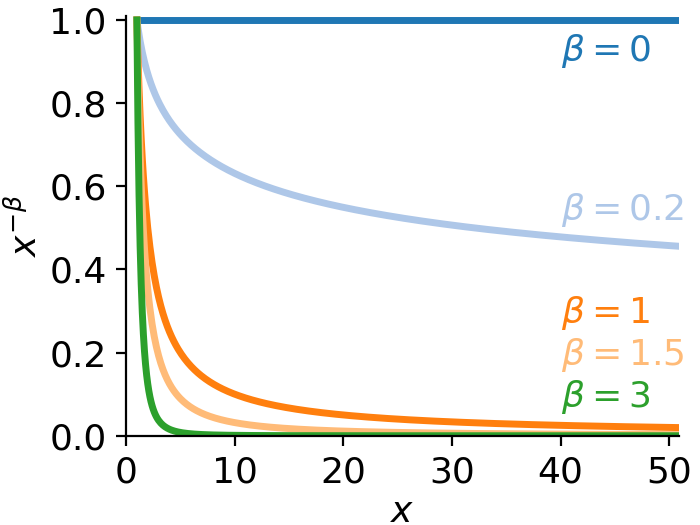
\includegraphics[scale=0.75]{images/generated/power-law}
    \caption{Power law functions.}
    \label{fig:power-law-functions}
\end{figure}

\begin{figure}
    \centering
    \subfloat{{
        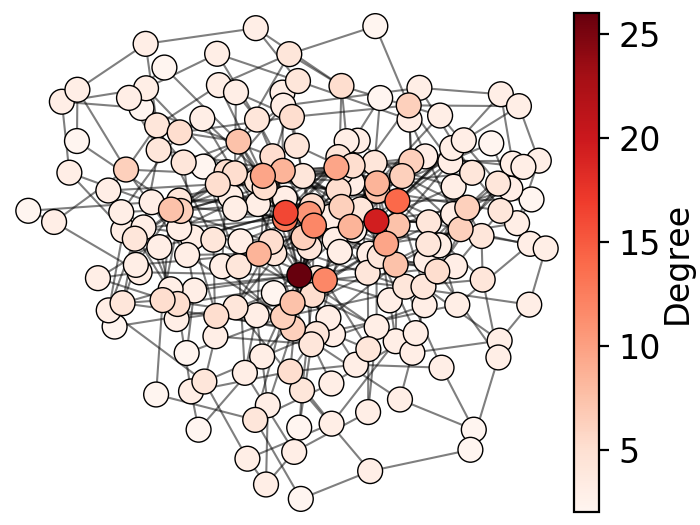
\includegraphics[scale=0.81]{images/generated/power-law-graph}
    }}
    \qquad
    \subfloat{{
        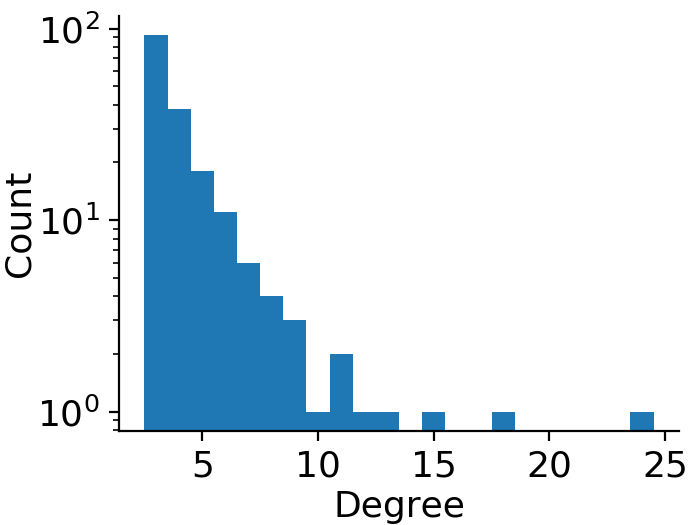
\includegraphics[scale=0.75]{images/generated/power-law-deg-distribution}
    }}
    \caption{Example of a power-law graph and its degree distribution.}
    \label{fig:power-law-graph-and-deg-distr}
\end{figure}

\begin{figure}
    \centering
    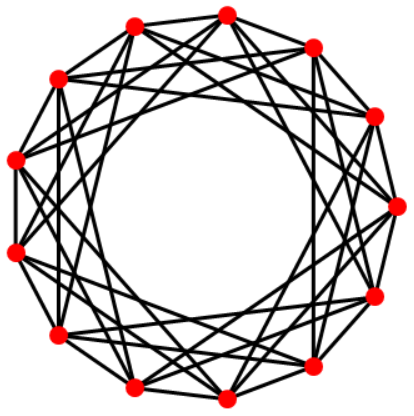
\includegraphics[width=0.35\textwidth]{images/paley}
    \caption{13-Paley graph is an example of an expander.}
    \label{fig:paley-graph}
\end{figure}

\section{Related Work}

The following results inspired us to look for expanders inside power-law graphs.

In~\cite{acl01} a random graph model for power-law graphs was introduced
and different properties were described, including connectivity and emergence of giant connected components.
This model is asymptotically equivalent to our coin toss model from~\autoref{sec:powerlaw-coin-toss-model}.
The difference is that our model defines the expected degree sequence
rather than the exact one, and that is crucial for our proof.

\cite{cl04} found the average distance in random graphs
with given expected degree sequences, both general and power-law with $2<\beta<3$.
The latter produces the ``octopus'' graphs described in~\autoref{sec:powerlaw-octopus-model}.

\cite{abl09} presented a power-law model which was shown to fit well
industrial SAT instances used in recent international competitions for SAT solvers.
They also focused on fitting the SAT instances,
i.e., estimating the appropriate distributions that would produce analogous degree sequences.
We talk about this model in~\autoref{sec:powerlaw-k-cnf-model}.

\cite{kri17} looked for a linearly sized expanders inside graphs
that are ``locally sparse'', as well as inside random $G(n,p)$ graphs.
The paper also contained the algorithm for actually finding the expanding subgraphs.

Finally, \cite{mst06} capitalized on the structure of power-law graphs
by displaying that one can discover the nodes via a random walk
with lookahead in sublinear time.
Considering~\cite{mih89}, this result also hints on possible expansion
properties of graphs with paths of constant length replaced by new edges.

As can be seen, there is a substantial amount of research done concerning separately
power-law models and expander graphs due to their wide popularity and usefulness.
One paper with significant steps made in the direction
of combining these two topics is~\cite{gms03}.
They consider random power-law graphs with the exponent $2<\beta<3$,
all vertices have degrees between $3$ and $O(\sqrt{n})$, and the volume is $O(n)$.
They also had to slightly modify graph construction from~\cite{acl01}
in order to ensure certain connectivity properties.
These graphs are shown to have conductance $\Theta(1)$,
which generalizes the notion of $(n/2,\Theta(1))$ edge expansion.

\begin{table}
    \begin{center}
        \renewcommand*{\arraystretch}{1.3}
        \begin{tabular}{|l|c|c|l|}
            \hline
            \multicolumn{1}{|c|}{Model} & \multicolumn{2}{|c|}{Object} & \multicolumn{1}{|c|}{Definition} \\
            \hline\hline
            Permutation model & \multirow{2}{*}{\vspace{-4mm}exact} & degrees & $\deg(i)=\frac{pn}{i^\beta}$\rule{0pt}{18pt}\\[0.6em]
            \cline{1-1}\cline{3-4}
            Model from~\cite{acl01} & & \multirow{2}{*}{{\renewcommand{\arraystretch}{1.0}\begin{tabular}{@{}l@{}}\\frequencies\\of degrees\end{tabular}}} & $|\{i \in V\;|\;\deg(i)=x\}|=\frac{e^\alpha}{x^\beta}$\rule{0pt}{18pt}\\[0.6em]
            \cline{1-2}\cline{4-4}
            Coin toss model & \multirow{2}{*}{\vspace{-4mm}expected} & & $\E_G[|\{i \in V\;|\;\deg(i)=x\}|]=\frac{e^\alpha}{x^\beta}$\rule{0pt}{18pt}\\[0.6em]
            \cline{1-1}\cline{3-4}
            Model from~\cite{cl04} & & degrees & $\E_G[\deg(i)]=w_i=ci^{-1/(\beta-1)},\;\beta>2$\rule{0pt}{18pt}\\[0.6em]
            \hline
        \end{tabular}
        \caption{Comparison of power-law graph models.}
        \label{tab:models-comparison}
    \end{center}
\end{table}

\section{Contribution of the Thesis}

We defined the models of power-law graphs, which would complement the ones studied earlier.
\autoref{tab:models-comparison} presents their comparison.
The permutation model was chosen so as to fit the uniformly random case when the exponent $\beta=0$.

The main result is that, under these models, the subgraphs containing
the vertices of sufficiently large degrees are edge or vertex expanders w.h.p.

More precisely, in the coin toss model, if $\beta<1$, actually the whole graph is an edge expander.
For $1\leq\beta\leq 1.6$ we have a linear size expanding subgraph,
and for $\beta>1.6$ the size of the expander is only $\Theta(n^{1/\beta})$.
In all the cases edge expansion is close to one half of the expected average degree $d$,
which is linear in the size of the subgraph.

In the permutation model, the case $\beta=0$ matches the previously known fact
that the whole graph has edge and vertex expansion almost $d-2$.
When $\beta>0$, we generalize the argument to show existence
of the edge expanders of size $n/2$ with expansion $d/2$,
but the average degree $d$ deteriorates for larger $\beta$.
Also, if $\beta>1$, there is an additional constraint $p\,\zeta(\beta)>2$
which essentially limits $\beta<1.72$.
Meanwhile, vertex expansion of the subgraph with vertices of degree
at least $d_0$ is almost $d_0/2-2$ whenever $\beta>0$.

Obtained results about linear size expanders inside power-law graphs
resemble existing result of the same nature for Erd\H{o}s-R\'enyi graphs~\cite{kri17}.
The size of our expanders is also comparable to the sizes of
the largest connected components in power-law graphs from~\cite{acl01}, i.e.,
we say that the largest components are not just connected, but ``highly connected''.
\autoref{tab:consistency-of-results} summarizes these details.

We proceed by showing that the core of the ``octopus'' graph with the vertices
of degree at least $n^{1/\log\log n}$ is an edge expander w.h.p.
and it contains a large vertex expander.

As a side result, we prove the logarithmic diameter of vertex expanders
with only small expanding subsets of size at most $\epsilon n$, for some
constant $\epsilon>0$, as opposed to $\epsilon=1/2$ in the canonical result.

To sum up, our findings provide better understanding of the structure
of power-law graphs from some general families for a wide range of parameters.
This knowledge can be further used to employ any techniques
applicable to expanders on these power-law graphs.

\begin{table}
    \begin{center}
        \renewcommand*{\arraystretch}{1.3}
        \begin{tabular}{|l|c|c|c|c|}
            \hline
            \multicolumn{1}{|r|}{$\beta$} & $(0;1.6)$ & $(1.6;1.72)$ & $(1.72;3.48)$ & $(3.48;\infty)$\\
            \hline\hline
            {\renewcommand{\arraystretch}{1.0}\begin{tabular}{@{}l@{}}The largest components\\in power-law graphs~\cite{acl01}\end{tabular}} & \multicolumn{3}{|c|}{the giant component, $\Theta(n)$} & $O\left(n^{2/\beta}\log n\right)$\rule{0pt}{19pt}\\[0.7em]
            \hline
            {\renewcommand{\arraystretch}{1.0}\begin{tabular}{@{}l@{}}Our edge expanders\\in coin toss model\end{tabular}} & $\Theta(n)$ & \multicolumn{3}{|c|}{$\Theta\left(n^{1/\beta}\right)$}\rule{0pt}{19pt}\\[0.7em]
            \hline\hline
            {\renewcommand{\arraystretch}{1.0}\begin{tabular}{@{}l@{}}Vertex/edge expanders\\in $G(n,p)$~\cite{kri17}\end{tabular}} & \multicolumn{4}{|c|}{$\Theta(n)$}\rule{0pt}{19pt}\\[0.7em]
            \hline
            {\renewcommand{\arraystretch}{1.0}\begin{tabular}{@{}l@{}}Our edge expanders\\in permutation model\end{tabular}} & \multicolumn{2}{|c|}{$\Theta(n)$} & \multicolumn{2}{|c|}{---}\rule{0pt}{19pt}\\[0.7em]
            \hline
        \end{tabular}
        \caption{Consistency of sizes between our results and the other papers.}
        \label{tab:consistency-of-results}
    \end{center}
\end{table}

\section{Our Methods}
%extra problems solved, difficulties encountered, our approach/methods/toolbox

For the coin toss model, we first obtain the necessary lower bounds
on the expected average degree. This is done by approximating
the expected size of an arbitrary cut, applying Chernoff concentration bounds,
and following the common argument for edge expansion.
Then we decide the size of an expanding subgraph and try to keep it linear
in the size of the whole graph by choosing an appropriate minimum degree
of vertices to be included in this subgraph.

While working with the permutation model, we adopt and generalize
the existing approaches from~\autoref{subsec:edge-expansion-reg}
and~\ref{subsec:vertex-expansion-reg}
for edge and vertex expansion of regular graphs.

Throughout this work, we deal with varying approximations of harmonic numbers,
so we have to treat different ranges of the exponent $\beta$ separately.

Lastly, our proof of small diameter of vertex expanders resembles
a common technique for graph decomposition.

\section{Thesis Structure}

In~\autoref{ch:prelims} we present all the necessary definitions,
approximations, and known results about expanders,
on which this research is based.
\autoref{ch:powerlaw} contains the detailed description
of the main models of power-law graphs used in this work.
In~\autoref{ch:expanders} we show the existence of expanding subgraphs
for the coin toss and permutation models,
and analyze the diameter of graphs with vertex expansion of small sets.
Finally, we compare the behavior of the random graphs
under different models in~\autoref{ch:comparison}, including their
diameters and sizes of expanders and connected components.

\chapter{Preliminaries}
\label{ch:prelims}

Here we explain the basic definitions as well as the notation used in the following chapters.

\section{Probability Theory and Inequalities}

We say an event $E(n)$ over a sample space $\Omega$
happens with high probability (w.h.p.) when:
\begin{equation}
    \lim_{n\to\infty}{\Pr_\Omega[E(n)]}=1
\end{equation}

\subsection{Union Bound}

If $\Omega$ is a sample space and $E_1,\ldots,E_n$ are events over $\Omega$, then:
\begin{equation}
    \Pr_\Omega\left[\bigcup_{i=1}^n{E_i}\right]\leq\sum_{i=1}^m{\Pr_\Omega\left[E_i\right]}
\end{equation}

\subsection{Chernoff Bounds}

% https://en.wikipedia.org/wiki/Chernoff_bound#Multiplicative_form_(relative_error)
Let $X_1,\ldots,X_n\in\{0,1\}$ be independent random variables,
and $X=\sum_{i=1}^n{X_i}$ with expected value
$\mu=\E[X]=\sum_{i=1}^n{\Pr[X_i=1]}$.
\begin{align}
    %\Pr[X\geq a]=\Pr[e^{tX}&\geq e^{ta}]\leq\frac{\E[e^{tX}]}{e^{ta}},\text{ for }t>0\\
    \Pr[X\geq(1+\delta)\mu]&\leq
    \begin{cases}
        \exp(-\delta^2\mu/(2+\delta)) & \quad \text{if } \delta>1,\\
        \exp(-\delta^2\mu/3) & \quad \text{if } 0<\delta\leq 1.
    \end{cases}\\
    \label{eq:chernoff-lower-tail}
    \Pr[X\leq(1-\delta)\mu]&\leq \exp(-\delta^2\mu/2),\text{ for }0<\delta<1
\end{align}
Combining these two we get:
\begin{equation}
    \label{eq:chernoff-combined}
    \Pr[|X-\mu|\geq\delta\mu]\leq 2\;\exp(-\delta^2\mu/3),\text{ for }0<\delta<1
\end{equation}

\subsection{Combinations}

\begin{equation}
    \left(\frac{n}{k}\right)^k
    \leq\binom{n}{k}=\frac{n!}{k!(n-k)!}
    \leq\left(\frac{en}{k}\right)^k
\end{equation}

It is easy to show:

$\frac{n}{k}\leq\frac{n-m}{k-m}$, for $0\leq m<k\leq n$,
so $\left(\frac{n}{k}\right)^k=\frac{n}{k}\ldots\frac{n}{k}$
$\leq\frac{n}{k}\frac{n-1}{k-1}\ldots\frac{n-k+1}{1}=\binom{n}{k}$

$\binom{n}{k}=\frac{n}{k}\frac{n-1}{k-1}\ldots\frac{n-k+1}{1}
\leq\frac{n^k}{k!}=\frac{k^k}{k!}\left(\frac{n}{k}\right)^k\leq\left(\frac{en}{k}\right)^k$

The last step uses the Maclaurin series of the exponential function:
\begin{equation}
    e^k=\sum_{n=0}^{\infty}{\frac{k^n}{n!}}\geq\frac{k^k}{k!}
\end{equation}

\subsection{Stirling's Approximation and the Number of Perfect Matchings}

Let $M(m)$ denote the number of perfect matchings on the set of even size $m$:
\begin{equation}
    M(m)=(m-1)!!=(m-1)(m-3)\ldots(3)(1)=\frac{m!}{2^{m/2}(m/2)!}
\end{equation}

We can use Stirling's approximation:
\begin{equation}
    \label{eq:stirling-approx}
    m!=(1+o(1))\sqrt{2\pi m}(m/e)^m
\end{equation}
\begin{equation}
    \label{eq:number-of-matchings}
    M(m)=(1+o(1))\frac{\sqrt{2\pi m}(m/e)^m}{2^{m/2}\sqrt{\pi m}(m/2e)^{m/2}}
    =(1+o(1))\sqrt{2}(m/e)^{m/2}
\end{equation}

\subsection{The Upper Bounds for the Sum of a Special Series}

The following sum $S_n$ occurs in several proofs. We will need to upper bound it
for $n\to\infty$ and some constants $0<\alpha\leq 1/2$, $c_1>0$, and $c_2>0$:
\begin{equation}
    S_n=\sum_{s=1}^{\alpha n}{\left(c_1(s/n)^{c_2}\right)^s}
\end{equation}
Each subsequent bound will require more rigorous analysis.

\begin{proposition}
    $S_n<1$, when $c_2\geq1+\log c_1$.
\end{proposition}

\begin{proof}
    $S_n=\sum_{s=1}^{\alpha n}{\left(c_1(s/n)^{c_2}\right)^s}
    \leq\sum_{s=1}^{\alpha n}{\left(c_1\alpha^{c_2}\right)^s}
    \leq\sum_{s=1}^{\infty}{2^{-c_3s}}
    \leq\sum_{s=1}^{\infty}{2^{-s}}<1$,
    where $c_3=c_2-\log c_1$ is a constant greater or equal $1$:
    \begin{gather}
        c_3\geq 1\iff c_2\geq 1+\log c_1\\
        c_1\alpha^{c_2}\leq c_1 2^{-c_2}=2^{-c_3}\leq 2^{-1}
    \end{gather}
\end{proof}

\begin{proposition}
    \label{pro:bound-prob-small-sets}
    $S_n\leq o(1)$ for some sufficiently small $\alpha$.
\end{proposition}

\begin{proof}
    First, we pick $\alpha$ so that $\left(c_1\alpha^{c_2}\right)<1/10$,
    using some constant $c_3>10$:
    \begin{equation}
        \alpha=(c_1c_3)^{-1/c_2}
    \end{equation}
    
    Then we consider small and large values of $s$ separately.
    Define $0<\epsilon<1$ such that:
    \begin{gather}
        \epsilon<(1-\epsilon)c_2\iff\epsilon<\frac{c_2}{1+c_2}\\
        S'=\sum_{s=1}^{n^\epsilon}{\left(c_1(s/n)^{c_2}\right)^s}
        \leq\sum_{s=1}^{n^\epsilon}{\left(\frac{c_1}{n^{(1-\epsilon)c_2}}\right)^s}
        \leq n^\epsilon\frac{c_1}{n^{(1-\epsilon)c_2}}=o(1)\\
        S''=\sum_{s=n^\epsilon+1}^{\alpha n}{(c_1(s/n)^{c_2})^s}
        <\sum_{s=n^\epsilon+1}^{\alpha n}{10^{-s}}
        \leq\frac{\alpha n}{10^{n^\epsilon}}=o(1)
    \end{gather}
    
    $S_n=S'+S''\leq o(1)$.
\end{proof}

\begin{proposition}
    \label{pro:bound-prob-large-sets}
    $S_n\leq o(1)$ for any $\alpha\leq 1/2$ and $c_2>\max\{1,\log c_1\}$.
    
    Moreover, $c_1$ and $c_2$ can be superconstants in terms of $n$,
    as long as $c_1=o\left(n^{c_2-1}\right)$.
\end{proposition}

\begin{proof}
    The argument is identical to the known one~\cite{gms03}.
    
    For $s\geq1$, let's define $f(s)=\left(c_1(s/n)^{c_2}\right)^s$, then
    $S_n=\sum_{s=1}^{\alpha n}{f(s)}$.
    The first two derivatives will help us understand the behavior of $f(s)$.
    
    First, the simple case when $c_1=c_2=1$:
    \begin{gather*}
        \frac{d}{ds}\left(\frac{s}{n}\right)^s
        =\frac{d}{ds}\exp\left(s\,\ln\frac{s}{n}\right)
        =\left(\frac{s}{n}\right)^s\left(\ln\frac{s}{n}+s\frac{1/n}{s/n}\right)
        =\left(\frac{s}{n}\right)^s\left(\ln\frac{s}{n}+1\right)\\
        \frac{d^2}{ds^2}\left(\frac{s}{n}\right)^s
        =\left(\frac{s}{n}\right)^s\left(\frac{1}{s}+\left(1+\ln\frac{s}{n}\right)^2\right)>0
    \end{gather*}
    We can see that $\left(\frac{s}{n}\right)^s$ is concave up for any $s\geq1$
    and attains its minimum at $s=n/e$.
    
    Then we perform similar steps for $f(s)$:
    \begin{equation}
        \begin{split}
            f'(s)=&\frac{d}{ds}\left(c_1\left(\frac{s}{n}\right)^{c_2}\right)^s
            =\frac{d}{ds}\exp\left(
                s\,
                \ln\left(c_1\left(\frac{s}{n}\right)^{c_2}\right)
            \right)=\\
            =&f(s)\left(
                \ln\left(c_1\left(\frac{s}{n}\right)^{c_2}\right)
                +s\frac{c_1c_2(s/n)^{c_2-1}(1/n)}{c_1(s/n)^{c_2}}
            \right)=\\
            =&f(s)\left(\ln\left(c_1\left(\frac{s}{n}\right)^{c_2}\right)+c_2\right)=\\
            =&f(s)c_2\left(\ln\frac{c_1^{1/c_2}s}{n}+1\right)=\\
            =&f(s)c_2\left(\ln\frac{s}{n}+\frac{\ln c_1}{c_2}+1\right)
        \end{split}
    \end{equation}
    \begin{equation}
        \begin{split}
            f''(s)=&\frac{d^2}{ds^2}\left(\frac{s}{n}\right)^s
            =\left(\frac{s}{n}\right)^s\left(\frac{1}{s}+\left(1+\ln\frac{s}{n}\right)^2\right)=\\
            % (3*((x/y)^7))^x * (log(3*((x/y)^7))+7)
            =&\frac{c_2}{s}f(s)+c_2\left(\ln\frac{s}{n}+1\right)f'(s)+(\ln c_1)f'(s)=\\
            =&\frac{c_2}{s}f(s)+c_2\left(\ln\frac{s}{n}+\frac{\ln c_1}{c_2}+1\right)f'(s)=\\
            =&\frac{c_2}{s}f(s)+\frac{(f'(s))^2}{f(s)}
        \end{split}
    \end{equation}
    
    Define $s_0$ to be an extreme point of $f(s)$:
    \begin{gather}
        f'(s_0)=0\\
        \ln\frac{c_1^{1/c_2}s}{n}=-1\\
        s_0=\frac{n}{ec_1^{1/c_2}}
    \end{gather}
    
    And verify that $f''(s)>0$ for any $s\geq1$:
    \begin{gather}
        \frac{c_2}{s}f(s)+\frac{(f'(s))^2}{f(s)}>0\\
        \frac{c_2}{s}+\left(\frac{f'(s)}{f(s)}\right)^2>0
    \end{gather}
    
    \begin{gather}
        \begin{cases}
            f'(s)<0 & \quad \text{if } s<s_0,\\
            f'(s)=0 & \quad \text{if } s=s_0,\\
            f'(s)>0 & \quad \text{if } s>s_0.
        \end{cases}\\
        f''(s)>0,\text{ for }s\in[1;\alpha n]
    \end{gather}
    
    Therefore, $f(s)$ is concave up on the whole interval
    $[1;\alpha n]$ with these endpoints:
    \begin{gather}
        f(1)=\frac{c_1}{n^{c_2}}\\
        f(\alpha n)=\left(c_1\alpha^{c_2}\right)^{\alpha n}
        \leq\left(c_1 2^{-c_2}\right)^{\alpha n}
    \end{gather}
    
    $f(1)=o(1/n)$ when $c_2>1$, and $f(\alpha n)=o(1/n)$
    when $c_1 2^{-c_2}<1\iff c_2>\log c_1$.
    
    Additionally, both $c_1$ and $c_2$ might be superconstants in terms of $n$,
    if this holds:
    \begin{equation}
        c_1=o\left(n^{c_2-1}\right)
    \end{equation}

    To sum up, given $c_2>\max\{1,\log c_1\}$:
    
    $S_n=\sum_{s=1}^{\alpha n}{f(s)}
    \leq\sum_{s=1}^{\alpha n}{\max\{f(1),f(\alpha n)\}}
    =o\left(\frac{\alpha n}{n}\right)=o(1)$.
\end{proof}

Note that if $c_2$ in~\autoref{pro:bound-prob-large-sets} is not large enough,
there is no advantage in terms of the size of expanding sets
compared to~\autoref{pro:bound-prob-small-sets}:
\begin{equation}
    c_1\alpha^{c_2}<1\iff\alpha<c_1^{-1/c_2}
\end{equation}

\section[Generalized Harmonic Numbers and Riemann Zeta Function]
        {Generalized Harmonic Numbers and Riemann Zeta\\Function}

Generalized harmonic numbers:
\begin{equation}
    H_{n,m}=\sum_{k=1}^{n}\frac{1}{k^m}
\end{equation}

We will extensively use these approximations for large $n$:
\begin{equation}
    H_{n,\beta}\approx
    \begin{cases}
        \frac{n^{1-\beta}}{1-\beta} & \quad \text{if } \beta<1,\\
        \ln n & \quad \text{if } \beta=1,\\
        \zeta(\beta) & \quad \text{if } \beta>1.
    \end{cases}
\end{equation}

The zeta function was introduced in 1737 by Euler, later Riemann allowed its argument to be a complex number.
\textit{Riemann zeta function} is defined for all $s\in\mathbb{C}$ with $\Re(s)>1$, see~\autoref{fig:zeta}:
\begin{equation}
    \label{eq:riemann-zeta-function}
    \zeta(s)=\sum_{n=1}^{\infty}\frac{1}{n^s}
\end{equation}
% https://math.stackexchange.com/q/876166
We know for $x\in\mathbb{R}$: $\zeta(x)\approx 1+2^{-x}$ when $x\gg 1$,
and $\lim_{x\to\infty}\zeta(x)=1$.

For $m>1$ as $n\to\infty$, applying the Euler-Maclaurin formula~\eqref{eq:euler-maclaurin-formula}
to the remainders $\sum_{n>N}{n^{-s}}$ of the sum~\eqref{eq:riemann-zeta-function}
provides the following connection:
\begin{gather}
    \zeta(s)=H_{N,s}+\frac{1}{(s-1)N^{s-1}}+\frac{1}{2N^s}+O\left(\frac{1}{N^{s+1}}\right),\quad\text{ for some }N\gg1\\
    H_{n,m}=\zeta(m)-\frac{1}{(m-1)n^{m-1}}-\frac{1}{2n^m}-O\left(\frac{1}{n^{m+1}}\right)
    =\zeta(m)-o(1)
\end{gather}

\begin{figure}
    \centering
    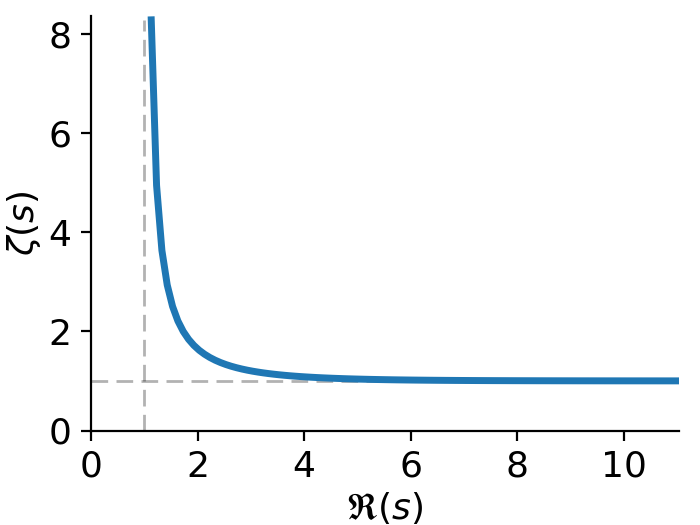
\includegraphics[scale=0.75]{images/generated/zeta}
    \caption[Riemann zeta function]{Riemann zeta function for $s\in\mathbb{C}$ with $\Re(s)>1$ and $\Im(s)=0$}
    \label{fig:zeta}
\end{figure}

\section{Gilbert and \texorpdfstring{Erd\H{o}s-R\'enyi}{Erdos-Renyi} Random Graphs}

The most commonly used models of uniform random graphs are $G(n,p)$ and $G(n,m)$
introduced by Gilbert~\cite{gil59} and by Erd\H{o}s and R\'enyi~\cite{er59}.

$G(n,p)$ contains all graphs where each pair of vertices
is connected by an edge with probability $p$.
We denote the maximum number of edges $N=\binom{n}{2}$,
then the expected number of edges in such graphs is $pN$.
\begin{gather}
    \Pr_{G\sim G(n,p)}[G\text{ has }m\text{ edges}]=\binom{N}{m}p^m(1-p)^{N-m}\\
    \Pr_{G\sim G(n,p)}[\deg(v)=k]=\binom{n-1}{k}p^k(1-p)^{n-k-1},\text{ for }v\in V(G)
\end{gather}

On the other hand, $G(n,m)$ describes the graphs with $n$ vertices and exactly $m$ edges.
Each of $\binom{N}{m}$ possible graphs is chosen uniformly at random.

Erd\H{o}s and R\'enyi~\cite{er60} depict the following structural properties of $G(n,p)$ graphs.
When $p=o(1/n)$, the graph is simply a disjoint union of trees.
Then consider the case $p=c/n$, where $c$ is some constant.
If $c<1$, the size of the largest component is just $O(\log n)$,
at the critical point $c=1$ its size is $\Theta\left(n^{2/3}\right)$,
and a unique giant component of size $\Theta(n)$ emerges when $c>1$.
Finally, the graphs are disconnected  w.h.p. when $p<(1-\epsilon)\log n/n$
and become connected w.h.p. when $p>(1+\epsilon)\log n/n$, for any $\epsilon>0$~\cite{er59}.

As per Chung and Lu~\cite{cl01,cl04}, the diameter of $G(n,p)$ is
$\Theta(\log n)$ when $p=c/n$, for some constant $c>1$,
and $(1+o(1))\frac{\log n}{\log np}$ if $p=\omega(1/n)$.
The diameter of a disconnected graph is assumed to be the maximum
diameter of its connected components.

%If $np\geq c>1$ for some constant $c$,
%and $\lim_{n\to\infty}{\frac{\log n}{\log np}}=\infty$,
%then the average distance of $G(n,p)$ is $(1+o(1))\frac{\log n}{\log np}$ w.h.p.~\cite{cl04}

If we choose $m=pN$, $G(n,p)$ and $G(n,m)$ models are almost identical for large $n$
and $p>\log n/n$, but some important properties might be different for smaller $p$.
For example, let $p=3/n$ and so $m=\frac{3}{2}(n-1)$.
In this case $G(n,p)$ is disconnected w.h.p., while $G(n,m)$ yields
a connected graph with high expansion~\cite{mah09} as almost 3-regular.

Independence of edges of $G(n,p)$ makes it similar to our coin toss model for power-law graphs,
and $G(n,m)$ corresponds more to $m$ edges model and permutation model,
which will be defined in~\autoref{ch:powerlaw}.

\section{Expander Graphs}

\subsection{Combinatorial Expansion}

First, we look at the combinatorial notions of expansion.

\begin{definition}
    A graph $G$ is called \textit{$(\alpha n,\gamma)$ edge expander} if for some $\gamma>0$:
    \begin{equation}
        \min_{\substack{S\subset V\\0<|S|\leq\alpha n}}\frac{|\partial S|}{|S|}\geq\gamma,
    \end{equation}
    where the left-hand side expression with $\alpha=1/2$ is \textit{the Cheeger constant $h(G)$}, and
    \begin{equation}
        \partial S=e(S,V\backslash S)=\{(u,v)\in E\;|\;u\in S,v\in V\backslash S\}.
    \end{equation}
\end{definition}

\begin{definition}
    Analogously, \textit{$(\alpha n,\gamma)$ vertex expander} satisfies the following condition:
    \begin{equation}
        \min_{\substack{S\subset V\\0<|S|\leq\alpha n}}\frac{|N_G(S)|}{|S|}\geq\gamma,
    \end{equation}
    where $N_G(S)$ is the external neighborhood of $S$ in $G$, i.e.,
    \begin{equation}
        N_G(S)=\{v\in V\backslash S\;|\;\exists u\in S, (u,v)\in E\}.
    \end{equation}
\end{definition}

\begin{definition}
    \textit{$(\alpha n,\gamma)$ unique-neighbor expander} is a graph satisfying:
    \begin{equation}
        \begin{split}
            \min_{\substack{S\subset V\\0<|S|\leq\alpha n}}
            \frac{|\{v\in V\backslash S\;|\;v\text{ is adjacent to exactly one }u\in S\}|}{|S|}\geq\gamma,\\
            \text{or }\min_{\substack{S\subset V\\0<|S|\leq\alpha n}}
            \frac{|\{v\in V\backslash S\;|\;\exists u\in S\;\forall w\in S ((v,w)\in E\longleftrightarrow w=u)\}|}{|S|}\geq\gamma.
        \end{split}
    \end{equation}
\end{definition}

\subsection{Spectral Expansion}

Let $\deg(v)$ be degree of the vertex $v$. Then the Laplacian of $G$ without loops or multiple edges~\cite{chu97}:
\begin{equation}
    \Laplacian=T^{-\frac{1}{2}}LT^{-\frac{1}{2}}
\end{equation}
where $T=diag(\deg(v))$,
\begin{align}
    L_{u,v}&=
    \begin{cases}
        \deg(v) & \quad \text{if } u=v \text{,}\\
        -1      & \quad \text{if } (u,v)\in E(G),\\
        0       & \quad \text{otherwise.}
    \end{cases}\\
    \Laplacian_{u,v}&=
    \begin{cases}
        1                                   & \quad \text{if } u=v \text{ and } \deg(v) \neq 0 \text{,}\\
        -\frac{1}{\sqrt{\deg(u)\deg(v)}}    & \quad \text{if } (u,v)\in E(G),\\
        0                                   & \quad \text{otherwise.}
    \end{cases}
\end{align}

%Nontrivial $G$~--- contains at least 1 edge.

When $G$ is \textit{d-regular}, $\Laplacian=I-\frac{1}{d}A$.

Let $g:V\to\mathbb{R}$ be an arbitrary function, $g=T^{1/2}f$,
and both $g$ and $f$ are viewed as column vectors.
The Rayleigh quotient:
\begin{equation}
    \frac{\langle g,\Laplacian g \rangle}{\langle g,g \rangle}
    =\frac{\sum_{u \sim v}{(f(u)-f(v))^2}}{\sum_{v}{f(v)^2\deg(v)}}
\end{equation}
%    d1 0 -1        d1f1-f3                                        d1=1
% f, 0  d2 0 f = f, d2f2     = f1(d1f1-f3)+f2(d2f2)+f3(-f1+d3f3) = d2=0 = d1f1^2-f1f3+d2f2^2+d3f3^2-f1f3
%    -1 0 d3        -f1+d3f3                                       d3=1

The eigenvalues of $\Laplacian$ (i.e., the spectrum of $G$) are $0=\lambda_1 \leq \lambda_2 \leq \dots \leq \lambda_{n}$.

Eigenvalue $0$ has eigenvector $T^{\frac{1}{2}}\mathbf{1}$.
% Laplacian*v=lambda*v=(0 0 ... 0)
% 1             0 -1/sqrt(d1d3)   sqrt(d1)   sqrt(d1)-1/sqrt(d1)   0
% 0             0 0             * sqrt(d2) = 0                   = 0
% -1/sqrt(d1d3) 0 1               sqrt(d3)   -1\sqrt(d3)+sqrt(d3)  0

The spectral expansion of $G$, also known as the spectral gap:

\begin{equation}
    \lambda_G=\lambda_2=\inf_{f \perp T^{\frac{1}{2}}\mathbf{1}}
    \frac{\sum_{u \sim v}{(f(u)-f(v))^2}}{\sum_{v}{f(v)^2\deg(v)}}
\end{equation}

%\begin{equation}
%    Tr(M)=\sum_v{M_{v,v}}=\sum_i{\lambda_i}
%\end{equation}
%
%The Laplacian of a weighted $G$:
%\begin{align}
%    L&=
%    \begin{cases}
%        \deg(v)-w(v,v)  & \quad \text{if } u=v \text{,}\\
%        -w(u,v)         & \quad \text{if } (u,v)\in E(G),\\
%        0               & \quad \text{otherwise.}
%    \end{cases}\\
%    \Laplacian&=
%    \begin{cases}
%        1-\frac{w(u,v)}{\deg(v)}                & \quad \text{if } u=v \text{ and } \deg(v) \neq 0 \text{,}\\
%        -\frac{w(u,v)}{\sqrt{\deg(u)\deg(v)}}   & \quad \text{if } (u,v)\in E(G),\\
%        0                                       & \quad \text{otherwise.}
%    \end{cases}
%\end{align}
%
%For $f:V\rightarrow\mathbb{R}$, $Lf(x)=\sum_{\substack{y\\x \sim y}}{(f(x)-f(y))w(x,y)}$

\subsection{Connections Between Different Types of Expansion}

Trivially, vertex expansion $\gamma_1$ implies edge expansion $\gamma_1$.
For $d$-regular graphs, edge expansion $\gamma_2$ implies vertex expansion $\gamma_2/d$.

The Cheeger inequalities~\cite{che69,hlw06,chu07} provide the link
between combinatorial and spectral expansion:
\begin{gather}
    \label{eq:cheeger-inequalities}
    \frac{h^2(G)}{2}\overset{(1)}{\leq}\lambda_G\overset{(2)}{\leq}2h(G),\\
    \text{or equivalently }\frac{\lambda_G}{2}\leq h(G)\leq\sqrt{2\lambda_G}
\end{gather}

\subsection{Construction of Expanders}

There are many ways to generate expander graphs:
algebraic constructions and zig-zag product~\cite{hlw06,vad12},
lifts~\cite{al06}, splicers and selectors~\cite{fgrv14},
local edge flips~\cite{ablmo16},
random coverings of a fixed good expander~\cite{pud15}, and so on.

In~\autoref{ch:expanders} we show yet another way~--- random power-law graphs
contain expanding induced subgraphs with vertices of large degrees.

\section{Expansion of Random Regular Graphs}

\begin{theorem}[Theorem 4.16~\cite{hlw06}]
    $\forall d\geq3\;\forall \delta>0\;\exists\gamma,\alpha>0$ such that
    a random $d$-regular graph on $n$ vertices is
    $(\alpha n,\gamma)$ edge expander and $(\alpha n,\gamma)$ vertex expander w.h.p.,
    $\gamma=d-2-\delta$.
\end{theorem}

\subsection{Vertex Expansion of Leftregular Bipartite Graphs}

Here $G$ is assumed to be a bipartite multigraph with $n$ vertices on each side.

\begin{definition}
    A graph $G$ is called \textit{$d$-leftregular}
    if each left-vertex is connected to exactly $d$ vertices from the right.
    In this case expansion is checked for all subsets $S$ of left-vertices.
\end{definition}

\begin{theorem}[\cite{vad12}]
    $\forall d\geq2\;\exists\alpha>0\;\forall n:$ a uniformly random $d$-leftregular $G$
    is $(\alpha n,d-2)$ vertex expander w.h.p.
\end{theorem}

\begin{proof}
    For a subset $S$ of a fixed size $s\leq\alpha n$ from the left side,
    $N_G(S)$ is a set of at most $sd$ vertices from the right labeled $v_1,v_2,\ldots,v_{sd}$.
    Then for every $v_i$:
    
    $\Pr_{G,S}[v_i\in N_G(S)\text{ is a repeat}]=\frac{\#\text{unique }v\text{'s in }\{v_1,\ldots,v_{i-1}\}}{n}
    \leq\frac{i-1}{n}\leq\frac{sd}{n}$
    
    $\Pr_{G,S}[|N_G(S)|\leq(d-2)s]\leq \Pr_{G,S}[\text{at least }2s\text{ repeats in }N_G(S)]
    \leq\binom{sd}{2s}\left(\frac{sd}{n}\right)^{2s}$
    
    $\Pr_G[\exists\text{ non-expanding }S]\leq\binom{n}{s}\binom{sd}{2s}\left(\frac{sd}{n}\right)^{2s}
    \leq\left(\frac{en}{s}\right)^s\left(\frac{esd}{2s}\right)^{2s}\left(\frac{sd}{n}\right)^{2s}
    =\left(\frac{e^3d^4s}{4n}\right)^s$
    
    Denote $c=(e^3d^4)/4$ and choose $\alpha=e^{-3}d^{-4}$, so that $c\alpha=1/4$.
    
    $\Pr_G[G\text{ is not }(\alpha n,d-2)\text{ vertex expander}]
    \leq\sum_{s=1}^{\alpha n}\left(c\frac{s}{n}\right)^{s}=o(1)$.
\end{proof}

\subsection{Edge Expansion of Regular Graphs}
\label{subsec:edge-expansion-reg}

\begin{theorem}[\cite{mag06}]
    \label{thm:reg-edge-expansion-optimal-gamma}
    $\forall d\geq3\;\forall\delta>0\;\exists\gamma,\alpha>0\;\forall\text{even }n:$
    a random $d$-regular graph $G=(V_G,E_G)$ is $(\alpha n,\gamma)$ edge expander w.h.p.,
    $\gamma=d-2-\delta$.
\end{theorem}

\begin{proof}
    Consider a new graph $H=(V_H,E_H)$ with $dn$ vertices
    and $E_H$ being a uniformly random perfect matching.
    Partition $V_H$ into sets $S_1,\ldots,S_n$ of size $d$,
    and identify the vertices from each $S_i$ with a single vertex $i$ in $G$.
    
    Let $S\subseteq V_G=\{1,\ldots,n\}$ be such that $|S|=s\leq\alpha n$.
    We can assume $S=\{1,\ldots,s\}$ and it is identified with $S_1\cup\ldots\cup S_{s}$.
    Then to pick $S$ we simply choose $ds$ vertices from $H$.
    
    To upper bound $|\partial(S)|$ we can lower bound the number of edges inside $S$.

    % ds/2 <= |e(S,S)| <= ds
    $\Pr_{G,S}[|e(S,V_G\backslash S)| < \gamma s] = \Pr_{G,S}\left[|e(S,S)|\geq\frac{(d-\gamma)s}{2}\right]
    \leq\frac{\binom{dn/2}{(d-\gamma)s/2}\binom{dn-(d-\gamma)s}{\gamma s}}{\binom{dn}{ds}}$
    
    $\Pr_G[G\text{ is not }(\alpha n,\gamma)\text{ edge expander}]
    \leq\sum_{s=1}^{\alpha n}{
        \binom{n}{s}
        \frac{
            \left(e\frac{dn}{(d-\gamma)s}\right)^{(d-\gamma)s/2}
            \left(e\frac{dn-(d-\gamma)s}{\gamma s}\right)^{\gamma s}
        }
        {\left(\frac{n}{s}\right)^{ds}}
    }=$

    $\qquad=\sum_{s=1}^{\alpha n}{
        \binom{n}{s}
        \frac{
            (edn)^{(d-\gamma)s/2}\;
            e^{\gamma s}\;
            (dn-(d-\gamma)s)^{\gamma s}\;
            s^{ds}
        }
        {
            ((d-\gamma)s)^{(d-\gamma)s/2}\;
            (\gamma s)^{\gamma s}\;
            n^{ds}
        }
    }\leq$

    $\qquad\leq\sum_{s=1}^{\alpha n}{
        \binom{n}{s}
        \frac{
            (ed)^{ds/2}\;
            (edn)^{\gamma s}\;
            s^{ds}
        }
        {
            (d-\gamma)^{(d-\gamma)s/2}\;
            (\gamma s)^{\gamma s}\;
            n^{ds}
        }
        \left(\frac{n}{s}\right)^{(d-\gamma)s/2}
    }=$

    $\qquad=\sum_{s=1}^{\alpha n}{
        \binom{n}{s}
        \frac{(ed)^{ds/2+\gamma s}}
        {
            (d-\gamma)^{(d-\gamma)s/2}\;
            \gamma^{\gamma s}
        }
        \left(\frac{s}{n}\right)^{(d-\gamma)s/2}
    }\leq$

    $\qquad\leq\sum_{s=1}^{\alpha n}{
        \frac{(ed)^{ds/2+\gamma s}}{(d-\gamma)^{(d-\gamma)s/2}}
        \left(\frac{e}{\gamma^\gamma}\right)^s
        \left(\frac{s}{n}\right)^{\left(\frac{d-\gamma}{2}-1\right)s}
    }=$

    $\qquad=\sum_{s=1}^{\alpha n}{\left(c_1\left(s/n\right)^{c_2}\right)^s}$,
    
    where $c_1=\frac{e(ed)^{d/2+\gamma}}{\gamma^\gamma(d-\gamma)^{(d-\gamma)/2}}\geq 0$
    and $c_2=\frac{d-\gamma}{2}-1$.
    
    We need $c_2>0$, which requires:
    \begin{equation}
        \gamma<d-2
    \end{equation}
    then by~\autoref{pro:bound-prob-small-sets}:
    
    $\Pr_G[G\text{ is not }(\alpha n,\gamma)\text{ edge expander}]=o(1)$.
\end{proof}

We will prove one of our results, \autoref{thm:powerlaw-permutation-edge-expansion}, in a similar fashion.

\begin{theorem}[\cite{bol88}]
    \label{thm:reg-edge-expansion-optimal-alpha}
    Let $d\geq3$ and $0<\epsilon<1$ be such that
    \begin{equation}
        \label{eq:bol-eps-req}
        (1-\epsilon)\log{(1-\epsilon)}+(1+\epsilon)\log{(1+\epsilon)}>4/d.
    \end{equation}
    Then any random $d$-regular graph $G$ has $h(G)\geq(1-\epsilon)d/2$ w.h.p.
\end{theorem}

The proof of this result uses the number of matchings
between endpoints of edges not crossing the cut $(S,V\backslash S)$.

Note that these two theorems sacrifice different parameters.
While \autoref{thm:reg-edge-expansion-optimal-gamma} shows how to achieve almost optimal expansion close to $d-2$,
only sufficiently small subsets are expanding.
On the contrary, \autoref{thm:reg-edge-expansion-optimal-alpha} talks about the Cheeger constant $h(G)$,
so the subsets may be as large as $n/2$, but the expansion might be as small as $d/2$.

%\begin{proof}
%    Let $P(s,k)=\Pr_G[\exists S:|e(S,V\backslash S)|=k]$, and $|S|=s$.
%    
%    Let $k_s$ be the largest integer less than $(1-\epsilon)ds/2$ such that $ds-k_s$ is even.
%    
%    $\Pr_G[G\text{ is not }(n/2,(1-\epsilon)d/2)\text{ edge expander}]
%    =\sum_{s=1}^{n/2}\sum_{\substack{0\leq k\leq k_s\\ds-k\text{ even}}}{P(s,k)}$
%    
%    $P(s,k)\leq P_0(s,k)=\binom{n}{s}\binom{ds}{k}\binom{dn-ds}{k}k!\frac{M(ds-k)M(dn-ds-k)}{M(dn)}$
%
%    where $M(m)$ is the number of matchings on $m$ elements, see~\eqref{eq:number-of-matchings}.
%    
%    For $2\leq k<k_s$: $P_0(s,k)<P_0(s,k+1)$, so it suffices to show that:
%    
%    $\sum_{s=1}^{n/2}\sum_{\substack{0\leq k\leq k_s\\ds-k\text{ even}}}{P_0(s,k)}
%    \leq\sum_{s=1}^{n/2}{k_s\,P_0(s,k_s)}=o(1)$
%    
%    Case 1: if $1\leq s\leq 100$, it is possible to verify that $P_0(s,k_s)=o(1)$.
%    
%    Case 2: for $100<s\leq n/2$ we will show $P_0(s,k_s)=o(n^{-2})$.
%    
%    There exists constant $K_d>0:P_0(s,k_s)\leq K_d P_0(n/2,k_{n/2})$.
%    
%    $P_0(n/2,k_{n/2})=\binom{n}{n/2}\binom{dn/2}{k_{n/2}}^2(k_{n/2})!\frac{(M(dn/2-k_{n/2}))^2}{M(dn)}$
%    
%    Using \eqref{eq:number-of-matchings} and the fact that $k_{n/2}\leq(1-\epsilon)dn/2$:
%    
%    $P_0(n/2,k_{n/2})=\ldots$
%    
%    $=o(1)\left(4d^d((1-\epsilon)d)^{-(1-\epsilon)d/2}((1+\epsilon)d)^{-(1+\epsilon)d/2}\right)^{n/2}$
%    
%    %todo it doesn't look right
%    $=o(1)\left(2^{4/d}(1-\epsilon)^{-(1-\epsilon)}(1+\epsilon)^{-(1+\epsilon)}\right)^{n/4d}$
%    
%    Finally, from the requirement \eqref{eq:bol-eps-req}:
%    
%    $P_0(n/2,k_{n/2})=o(1)$.
%\end{proof}

\subsection{Vertex Expansion of Regular Graphs}
\label{subsec:vertex-expansion-reg}

\begin{theorem}[\cite{rao12}]
    \label{thm:reg-vertex-expansion}
    $\forall d\geq3\;\forall\delta>0\;\exists\gamma,\alpha>0\;\forall\text{even }n:$ a random $d$-regular graph $G=(V,E)$
    is $(\alpha n,\gamma)$ vertex expander w.h.p., $\gamma=d/2-2-\delta$.
\end{theorem}

\begin{proof}
    Let $E$ be the union of $d$ uniformly random perfect matchings.
    
    For any subset $S$ of size $|S|=s\leq\alpha n$,
    and any subset $T$ of $(1+\gamma)s$ vertices we will bound the probability that
    $N_G(S)\subseteq T$ under one of the perfect matchings.
    
    Any fixed perfect matching $E'\subset E$ might be viewed as connecting one pair of
    unmatched vertices sequentially, until every vertex has a match.
    Let $E_i$ denote the event that $i$'th vertex in $S$ is matched to some vertex in $T$ under $E'$.
    Of course, $E_i$ is well defined only for $i\leq\ceil{\frac{s}{2}}$.
    For the sake of simplicity, lets assume $s$ is even.
    
    $\Pr_{G,S,T,E'}\left[\bigwedge\limits_{i=1}^{s/2}{E_i}\right]
    =\prod_{i=1}^{s/2}{\Pr_{G,S,T,E'}\left[E_i\;\middle|\;\bigwedge\limits_{k=1}^{i-1}{E_k}\right]}
    \leq\prod_{i=1}^{s/2}{\Pr_{G,S,T,E'}[E_i]}\leq\left(\frac{(1+\gamma)s}{n}\right)^{s/2}$
    
    $\Pr_{G,S,T}[N_G(S)\subseteq T]\leq\left(\frac{(1+\gamma)s}{n}\right)^{sd/2}$
    
    $\Pr_G[\exists\text{ non-expading }S\text{ of size }s]
    \leq\binom{n}{s}\binom{n}{(1+\gamma)s}\left(\frac{(1+\gamma)s}{n}\right)^{sd/2}\leq$

    $\qquad\leq\left(\frac{en}{s}\right)^s\left(\frac{en}{(1+\gamma)s}\right)^{(1+\gamma)s}\left(\frac{(1+\gamma)s}{n}\right)^{sd/2}
    =\left(\frac{(en)^{2+\gamma}((1+\gamma)s)^{d/2}}
    {n^{d/2}(1+\gamma)^{1+\gamma}s^{2+\gamma}}\right)^s=$
    
    $\qquad=\left(e^{2+\gamma}(1+\gamma)^{d/2-1-\gamma}\left(\frac{s}{n}\right)^{d/2-2-\gamma}\right)^s=$
    
    $\qquad=\left(c_1\left(s/n\right)^{c_2}\right)^s$.
    
    We need $c_2>0$, which requires $\gamma<d/2-2$.
    For sufficiently small $\alpha$:
    
    $\Pr_G[G\text{ is not }(\alpha n,\gamma)\text{ vertex expander}]
    \leq\sum_{s=1}^{\alpha n}{(c_1(s/n)^{c_2})^s}=o(1)$.
\end{proof}

\section{Edge Expansion of Random Graphs With Given Degrees}

Gkantsidis et al.~\cite{gms03} deal with the power-law graphs
and their model is based on the one from Aiello et al.~\cite{acl01}.
However, this following result holds for random graphs with general degree sequences.

\begin{theorem}[Lemma 3.2~\cite{gms03}]
    \label{thm:gms}
    Let $(w_1,\ldots,w_n)$ be a sequence of integers and
    \begin{gather}
        w_1\geq w_2\geq \ldots\geq w_n\geq d_{min}=3\\
        D=\sum_{i=1}^{n}{w_i} %=O(n) unused
    \end{gather}
    Let $G=(V,E)$ be a random graph with a degree sequence $(w_1,\ldots,w_n)$
    generated according to the permutation model of~\autoref{subsec:permutation-model}.
    Then there is a constant $\gamma>0$, which satisfies
    \begin{equation}
        \begin{cases}
            \gamma<1-2/d_{min}\\
            \gamma\leq1-8/(3\,d_{min})\\
            \gamma\leq 0.0175
        \end{cases}\implies
        \gamma=0.0175
    \end{equation}
    such that w.h.p.
    \begin{equation}
        % conductance=
        \min_{\substack{S\subset V\\0<\vol(S)\leq D/2}}
        \frac{|e(S,V\backslash S)|}{\vol(S)}\geq\gamma=\Omega(1)
    \end{equation}
\end{theorem}

\begin{proof}
    For a constant $\gamma>0$ a set $S$ with $\vol(S)\leq D/2$ is called ``bad''
    if $\frac{|e(S,V\backslash S)|}{\vol(S)}<\gamma$.
    
    We will show that for some $\gamma$, $\Pr_G[\exists\text{ bad }S]\leq o(1)$.
    
    $\Pr_G[\exists\text{ bad }S]
    =\sum_{k=d_{min}}^{D/2}{\Pr_G[\exists\text{ bad }S,\vol(S)=k]}\leq$
    
    $\qquad\leq\sum_{k=d_{min}}^{D/2}{\binom{D/d_{min}}{k/d_{min}}\Pr_G[\text{a fixed }S,\vol(S)=k\text{, is bad}]}$.
    
    Let $A$ denote a set of $k$ mini-vertices corresponding to $S$,
    and $\bar{A}$ to be $(D-k)$ mini-vertices that correspond to $V\backslash S$.
    Let $B_A\subset A$ be a set of mini-vertices matched to the ones from $\bar{A}$,
    and similarly $B_{\bar{A}}\subset\bar{A}$ is matched to some mini-vertices from $A$.
    $S$ is ``bad'' when $|B_A|=|B_{\bar{A}}|<\gamma k$.
    For each cardinality from $0$ to $\gamma k$, there are at most
    $\binom{k}{\gamma k}$ and $\binom{D-k}{\gamma k}$ ways
    to choose $B_A$ and $B_{\bar{A}}$ respectively.
    Then we consider a random perfect matchings
    with all mini-vertices from $A\backslash B_A$ matched inside $A\backslash B_A$,
    and the same for $\bar{A}\backslash B_{\bar{A}}$ and $B_A\cup B_{\bar{A}}$.
    
    $\Pr_G[\exists\text{ bad }S]\leq\sum_{k=d_{min}}^{D/2}{
        \binom{D/d_{min}}{k/d_{min}}\gamma k\binom{k}{\gamma k}\binom{D-k}{\gamma k}
        \frac{M(2\gamma k)\,M(k-\gamma k)\,M(D-k-\gamma k)}{M(D)}
    }$

    We will use the approximation~\eqref{eq:number-of-matchings}
    for the number of perfect matchings on $m$ vertices,
    where $c_1$ and $c_2$ are some positive constants:
    \begin{equation}
        c_1(m/e)^{m/2}<M(m)<c_2(m/e)^{m/2}
    \end{equation}

    $\gamma k\frac{M(2\gamma k)\,M(k-\gamma k)\,M(D-k-\gamma k)}{M(D)}<$
    
    $\qquad<c_4\gamma k
    \left(\frac{2\gamma k}{e}\right)^{\gamma k}
    \left(\frac{k-\gamma k}{e}\right)^{(k-\gamma k)/2}
    \left(\frac{D-k-\gamma k}{e}\right)^{(D-k-\gamma k)/2}
    \left(\frac{e}{D}\right)^{D/2}=$
    
    $\qquad=c_4\gamma k\frac{
        (2\gamma k)^{\gamma k}\,
        (k-\gamma k)^{(k-\gamma k)/2}\,
        (D-k-\gamma k)^{(D-k-\gamma k)/2}
    }{D^{D/2}}<$

    $\qquad<c_4\gamma k\,(2\gamma)^{\gamma k}\,\frac{
        k^{(k+\gamma k)/2}\,
        (D-k)^{(D-k-\gamma k)/2}
    }{D^{D/2}}$.

    We apply Stirling's approximation~\eqref{eq:stirling-approx},
    for some constant $c_3>0$:

    $\binom{D/d_{min}}{k/d_{min}}=\frac{(D/d_{min})!}{(k/d_{min})!((D-k)/d_{min})!}<$
    
    $\qquad<\Theta(1)
    \left(\frac{D}{d_{min}}\right)^{D/d_{min}+1/2}
    \left(\frac{d_{min}}{k}\right)^{k/d_{min}+1/2}
    \left(\frac{d_{min}}{D-k}\right)^{(D-k)/d_{min}+1/2}\leq$
    
    $\qquad\leq c_3\left(\frac{D^D}{k^k(D-k)^{D-k}}\right)^{1/d_{min}}$.
    
    Finally, we use $\binom{n}{m}\leq(en/m)^m$:
    \begin{equation*}
        \binom{k}{\gamma k}\binom{D-k}{\gamma k}
        \leq\left(\frac{e}{\gamma}\right)^{2\gamma k}\left(\frac{D-k}{k}\right)^{\gamma k}
    \end{equation*}
    
    Let's combine all of the above:
    
    $\Pr_G[\exists\text{ bad }S]<\sum_{k=d_{min}}^{D/2}{c_5\gamma k
    \frac{2^{\gamma k}e^{2\gamma k}}{\gamma^{\gamma k}}
    \left(\frac{k}{D}\right)^{k((1-\gamma)/2-1/d_{min})}}$
    
    Define $\alpha=\frac{2e^2}{\gamma}$,
    $\beta=\frac{1-\gamma}{2}-\frac{1}{d_{min}}$, and
    \begin{equation}
        G(k)=c_5\gamma k\alpha^{\gamma k}\left(\frac{k}{D}\right)^{\beta k}
    \end{equation}
    We require $\beta>0$, which means $d_{min}>\frac{2}{1-\gamma}$,
    so $d_{min}\geq3$. Also $\gamma<1-\frac{2}{d_{min}}$.
    \begin{gather}
        \frac{dG(k)}{dk}=\left(\frac{1}{k}+\gamma\ln\alpha+\beta\ln\frac{k}{D}+\beta\right)\,G(k)\\
        \frac{d^2G(k)}{dk^2}=\left(-\frac{1}{k^2}+\frac{\beta}{k}+\left(\frac{dG(k)}{dk}\right)^2\right)\,G(k)
    \end{gather}
    
    $dG(k)/dk<0$ for $k=3\,d_{min}$ when $D$ is large.
    
    $d^2G(k)/dk^2>0$ for $k\geq3\,d_{min}$ and $\gamma\leq1-8/(3\,d_{min})$. %todo ?
    
    Clearly, $\sum_{k=d_{min}}^{3\,d_{min}}{G(k)}=o(1)$.
    
    To upper bound the sum for $3\,d_{min}\leq k\leq D/2$,
    we can use $\max\{G(3\,d_{min}),G(D/2)\}$.
    \begin{gather}
        G(3\,d_{min})=c_6D^{-3\,d_{min}\beta}=o\left(\frac{1}{D}\right)\\
        G(D/2)=c_7D\left(\frac{\alpha^\gamma}{2^\beta}\right)^{D/2}=o\left(\frac{1}{D}\right)
    \end{gather}
    for constants $c_6$, $c_7$, and
    \begin{gather}
        \begin{cases}
            3\,d_{min}\beta>1\\
            \alpha^\gamma<2^\beta
        \end{cases}\implies
        \begin{cases}
            \gamma\leq1-8/(3\,d_{min})\\
%            \gamma\log{\alpha}<\beta
            \gamma(\frac{1}{2}+2\log_2{e}-\log_2{\gamma})<\frac{1}{2}-\frac{1}{d_{min}}
        \end{cases}
    \end{gather}
    If $d_{min}=3$, the last inequality holds whenever $\gamma\leq 0.0175$.
    
    $\Pr_G[\exists\text{ bad }S]<\sum_{k=d_{min}}^{3\,d_{min}}{G(k)}
    +\sum_{k=3\,d_{min}}^{D/2}{G(k)}\leq o(1)$.
\end{proof}

\section{Vertex Expanders in Locally Sparse Graphs and \texorpdfstring{$G(n,p)$}{G(n,p)}}

For a graph $G=(V,E)$ on $n$ vertices and a subset $W\subseteq V$ set $\vol(W)=\sum_{v\in W}\deg(v)$.

\begin{theorem}[\cite{kri17}]
    \label{thm:kri}
    Let $c_1>c_2>0, 0<\alpha<1, \Delta>0$, and
    $G=(V,E), \Delta(G)\leq\Delta,\frac{|E|}{|V|}\geq c_1$.
    Then there exist a constant $\gamma=\gamma(c_1,c_2,\alpha,\Delta)>0$
    and poly$(n)$-time algorithm that finds
    either $W\subset V$ of size $|W|\leq\alpha n$ spanning at least $c_2|W|$ edges,
    or an induced $(|W|/2,\gamma)$ vertex expander on $|W|\geq\alpha n$ vertices.
\end{theorem}

\begin{proof}[Proof outline]
    The idea is to begin with $G$ and iteratively decrease
    the number of vertices, while maintaining the density.
    See~\autoref{alg:kri} for details.
\end{proof}

\begin{proposition}[\cite{kri17}]
    \label{pro:kri-1}
    Let $c_1>c_2>1$ be reals. Define $\alpha=\left(\frac{c_2}{5c_1}\right)^{c_2/(c_2-1)}$.
    Let $G$ be a random graph drawn from the probability distribution $G\left(n,\frac{c_1}{n}\right)$.
    Then w.h.p. every set of $k\leq\alpha n$ vertices of $G$ spans fewer than $c_2k$ edges.
\end{proposition}

\begin{proposition}[\cite{kri17}]
    \label{pro:kri-2}
    For every $c>0$ and all sufficiently small $\delta>0$ the following holds.
    Let $G$ be a random graph drawn from the probability distribution $G\left(n,\frac{c}{n}\right)$.
    Then w.h.p. every set of $\frac{\delta}{\ln 1/\delta}n$ vertices of $G$ touches fewer than $\delta n$ edges.
\end{proposition}

\begin{theorem}[Linear size expanders in $G(n,p)$ graphs~\cite{kri17}]
    \label{thm:kri-gnp}
    $\forall\epsilon>0\;\exists\gamma>0:$ a random graph $G\sim G\left(n,\frac{1+\epsilon}{n}\right)$
    contains w.h.p. an induced bounded degree $(n'/2,\gamma)$ vertex expander
    on $n'\geq\gamma n$ vertices.
\end{theorem}

\begin{proof}[Proof outline]
    A known fact about $G\left(n,\frac{1+\epsilon}{n}\right)$ is the existence of a giant connected component with ``enough'' edges.
    Removing a constant fraction of vertices having the highest degree, we get the bounded maximum degree by \autoref{pro:kri-2}.
    Then \autoref{pro:kri-1} guarantees the local sparsity, and we apply \autoref{thm:kri}.
\end{proof}

\chapter{Random Power-Law Graphs}
\label{ch:powerlaw}

\section{Models of Graphs}

We will work with models of graphs that define either degree sequences or frequencies of degrees.
In the latter case one can easily obtain the degree sequence as well,
e.g., the frequencies $(x_1,x_2,x_3)=(2,1,4)$ would be transformed into the degrees $(1,1,2,3,3,3,3)$.

Given a degree sequence $(w_1,\ldots,w_n)$, there are several ways to generate corresponding random graphs $G=(V,E)$~\cite{hop08}.
Depending on the particular model, this will be either exact (fixed) or expected degree sequence.

All subsequent models possibly result in pseudographs --- multigraphs with self-loops.
Therefore, the degree sequences are only required to be pseudographic:
degrees must be non-negative, and in case of exact degrees, they should add up to an even number~\cite{hak62}.

\subsection{Coin Toss Model}
\label{subsec:coin-toss-model}

For each pair of vertices $i$ and $j$, we include the edge $(i,j)$ in the graph with probability
\begin{equation}
    p_{ij}=\Pr_G[(i,j)\in E]=
    \begin{cases}
        \frac{w_i w_j}{\sum_{k\in V}{w_k}} & \quad \text{if }i\neq j,\\
        \frac{w_i^2}{2\sum_{k\in V}{w_k}} & \quad \text{otherwise}.
    \end{cases}
\end{equation}
Given expression is a valid probability, if we have
\begin{equation}
    \label{eq:coin-toss-assumption}
    \max_k w_k^2<\sum_{k\in V}{w_k}
\end{equation}
% http://mathworld.wolfram.com/GraphicSequence.html
This assumption also implies that the sequence is graphic,
i.e., realizable by some graph.

The standard convention is that self-loop edges contribute 2 to the degrees of the nodes.
Considering this, we show that the model is well-defined:
\begin{equation}
    \E_G[\deg(i)]=\sum_{j\neq i}{p_{ij}}+2p_{ii}
    =\frac{\sum_{j\neq i}{w_i w_j}+w_i^2}{\sum_{j\in V}{w_j}}=w_i
\end{equation}

Alternatively, one can generate a graph by including some number of edges between $i$ and $j$
according to a Poisson process with mean $\lambda=\frac{w_i w_j}{\sum_{k\in V}{w_k}}$.
High degree vertices would then form a clique.

In this model all edges are independent, and $(w_1,\ldots,w_n)$ are the expected degrees.

\subsection{\texorpdfstring{$m$}{m} Edges Model}

We generate $m=\frac{1}{2}\sum_{k\in V}{w_k}$ edges uniformly at random
by successively selecting pairs of vertices with probability proportional to their degrees.
In this case $w_i$'s are also expected degrees, however, we get
the exact number of edges, which are no longer independent.

\subsection{Permutation Model}
\label{subsec:permutation-model}

We create a sequence with $w_i$ mini-vertices for each vertex $i$,
randomly permute it, and connect each consecutive
non-intersecting pair of mini-vertices with an edge.
Equivalently, one can choose a uniformly random perfect matching on this sequence.
Then we put an edge between vertices $i$ and $j$ if at least one pair
of mini-vertices corresponding to both of them is adjacent.

This model guarantees the exact number of edges and they are not independent,
but the degree sequence is now exact.

\subsection{Full Graph Selection Model}

We randomly pick a graph $G$ from a family of all graphs with given
exact degree sequence, but it is usually not practical.

In this chapter we will examine the properties of power-law graphs under different models.

\section{Coin Toss Power-Law Model}
\label{sec:powerlaw-coin-toss-model}

We are given the expected degree sequence $(w_1,\ldots,w_n)$, where $w_v=\E[\deg(v)]$.
\begin{gather}
    \label{eq:powerlaw-coin-toss-edge-pr}
    \Pr_G[(u,v)\in E]=\frac{w_u w_v}{\Vol(G)},
    \quad\text{ assuming }\max_v w_v^2<\Vol(G)\\
    \Vol(G)=\E_G[\vol(G)]=\E_G\left[\sum_{v\in V} \deg(v)\right]=\sum_{v\in V} w_v
\end{gather}

%Note that by~\eqref{eq:chernoff-combined}: $\Pr_G[|\vol(G)-\Vol(G)|\geq\delta]\leq2\,\exp(-\delta^2/(3\;\Vol(G)))$.

Let the expected number of vertices with degree $x$ be equal to $y$,
which follows the power-law distribution for some $\alpha=\alpha(n)>0$ and constant $\beta>0$.
Note that $\alpha$ and $\beta$ are the only open parameters is this model.
\begin{equation}
    \E_G[|\{v \in V\;|\;\deg(v)=x\}|]=y=\frac{e^\alpha}{x^\beta},
    \quad\text{where }x\in\{1,\ldots,d_{max}\}.
\end{equation}

Our model is asymptotically identical to Aiello et al.~\cite{acl01},
whose properties are summarized in~\autoref{tab:graphs-properties-acl01}.
The only distinction is in defining the expected frequencies instead of the exact ones.

\begin{table}
    %\begin{shaded}
    \begin{center}
        \caption[Properties of power-law graphs~\cite{acl01}]
                {Properties of power-law graphs~\cite{acl01}, $\beta_0\approx3.4785$}
        \label{tab:graphs-properties-acl01}
        \renewcommand*{\arraystretch}{1.3}
        \begin{tabular}{|l|c|c|c|c|c|c|}
            \hline
            \multicolumn{1}{|r|}{$\beta$} & $(0;1)$ & $1$ & $(1;2)$ & $2$ & $(2;\beta_0)$ & $(\beta_0;\infty)$\\
            \hline\hline
            {\renewcommand{\arraystretch}{1.0}\begin{tabular}{@{}l@{}}the largest\\component\end{tabular}} & $n$ & \multicolumn{4}{|c|}{the giant component, $\Theta(n)$} & \multirow{2}{*}{\vspace{-4mm}$O\left(n^{2/\beta}\log n\right)$}\rule{0pt}{19pt}\\[0.7em]
            \cline{1-6}
            {\renewcommand{\arraystretch}{1.0}\begin{tabular}{@{}l@{}}the 2nd largest\\component\end{tabular}} & --- & \multicolumn{2}{|c|}{$O(1)$} & $O\left(\frac{\log n}{\log\log n}\right)$ & $O(\log n)$ &\rule{0pt}{20pt}\\[0.7em]
            \cline{1-7}
            $|V|=n$ & $\frac{e^{\alpha/\beta}}{1-\beta}$ & $\alpha e^\alpha$ & \multicolumn{4}{|c|}{$\zeta(\beta)e^\alpha$}\rule{0pt}{21pt}\\[0.7em]
            \cline{1-7}
            $|E|$ & \multicolumn{3}{|c|}{$\frac{1}{2}\frac{e^{2\alpha/\beta}}{2-\beta}$} & $\frac{1}{4}\alpha e^\alpha$ & \multicolumn{2}{|c|}{$\frac{1}{2}\zeta(\beta-1)e^\alpha$}\rule{0pt}{21pt}\\[0.7em]
            \hline
        \end{tabular}
    \end{center}
    %\end{shaded}
\end{table}

\subsection{Maximum Degree, Expected Size, and the Number of Edges}

Like Aiello et al.~\cite{acl01}, we ignore isolated vertices, $y\geq1$
and $0\leq\ln y=\alpha-\beta\ln x$, consequently, we may deduce
\begin{equation}
    d_{max}=e^{\alpha/\beta}
\end{equation}

The size of the graph and the expected number of edges are
\begin{equation}
    \label{eq:powerlaw-coin-toss-n-e}
    n=\sum_{x=1}^{e^{\alpha/\beta}}{\frac{e^\alpha}{x^\beta}}
    \qquad \E_G[|E|]=\frac{\Vol(G)}{2}=\frac{1}{2}\sum_{x=1}^{e^{\alpha/\beta}}{x\frac{e^\alpha}{x^\beta}}
\end{equation}

%These values of $d_{max}$ and $\Vol(G)$ do not satisfy~\eqref{eq:coin-toss-assumption}:
%
%$d_{max}^2=e^{2\alpha/\beta}>\Vol(G)$, when $0<\beta<1$ or $\beta=2$
%
%Erd\H{o}s-Gallai theorem (for simple graphs with integer $w_i$'s) gives the necessary and sufficient condition:
%$\sum_{i=1}^{k}{w_i}\leq k(k-1)+\sum_{i=k+1}^{n}{\min(w_i,k)}$.
%
%The number of edge-vertex adjacencies among $k$ vertices of the highest degree$\leq\ldots$
%
%$n-1\geq w_1\geq w_2\geq\ldots\geq w_n$,
%$\sum_{i=1}^n{w_i}$ is even

To get some intuition about the density of $G$,
we consider the special case when $d_{max}=n$.
\begin{gather}
    n=\sum_{x=1}^{n}\frac{e^\alpha}{x^\beta}=e^\alpha H_{n,\beta} \qquad e^\alpha=\frac{n}{H_{n,\beta}}\\
    \E_G[m]=\frac{1}{2}\E_G[\sum_{v \in V}\deg(v)]=\frac{1}{2}\sum_{x=1}^{n}x\frac{e^\alpha}{x^\beta}
    =\frac{e^\alpha}{2}\sum_{x=1}^{n}x^{1-\beta}=\frac{e^\alpha}{2}H_{n,\beta-1}
    =\frac{n}{2}\frac{H_{n,\beta-1}}{H_{n,\beta}}
\end{gather}

$H_{n,-1}=\frac{n(n+1)}{2},
\qquad H_{n,0}=n,
\qquad H_{n,1}=\log n+O(1),
\qquad H_{n,\beta}=O(1)\text{, if }\beta>1.$

\begin{equation}
    \E_G[m]=
    \begin{cases}
        \Theta\left(n^2\right) & \quad \text{if } \beta=0,\\
        \Theta\left(n^2/\log n\right) & \quad \text{if } \beta=1,\\
        \Theta(n\log n) & \quad \text{if } \beta=2,\\
        \Theta(n) & \quad \text{if } \beta>2.
    \end{cases}
\end{equation}

\subsection{Expected Volume and Average Degree}

When $n\to\infty$, the expected volume $\Vol(G)$ is well-defined only for $\beta>2$.
\begin{gather}
    \Vol(G)\approx\int_1^{\infty}{x\frac{e^\alpha}{x^\beta}}\,dx
    =\frac{e^\alpha}{2-\beta}\left[ x^{-\beta+2} \right]_1^\infty
    =\frac{e^\alpha}{\beta-2}
\end{gather}
On the other hand, considering $d_{max}=e^{\alpha/\beta}$ we get
\begin{equation}
    \label{eq:powerlaw-coin-toss-vol}
    \Vol(G)\approx\frac{e^\alpha}{2-\beta}\left(\left(e^{\alpha/\beta}\right)^{-\beta+2}-1\right)
    =\frac{1}{2-\beta}\left(e^{2\alpha/\beta}-e^\alpha\right)
\end{equation}
The expected average degree is
\begin{equation}
    d=\frac{\Vol(G)}{n}
\end{equation}
The second-order average degree is
\begin{equation}
    \tilde{d}=\frac{\sum_{v\in V}{w_v^2}}{\Vol(G)}\approx
    \begin{cases}
        d\frac{(\beta-2)^2}{(\beta-1)(\beta-3)} & \quad \text{if } \beta>3\\
        \frac{1}{2}d\ln \frac{2d_{max}}{d} & \quad \text{if } \beta=3\\
        d^{\beta-2}\frac{(\beta-2)^{\beta-1}d_{max}^{3-\beta}}{(\beta-1)^{\beta-2}(3-\beta)} & \quad \text{if } 2<\beta<3
    \end{cases}
\end{equation}

%\subsection{The Least and the Most Popular Vertices}
%
%$L_c = \{c\text{ least popular vertices}\}, M_c = \{c\text{ most popular vertices}\}$
%OR "vertices w/ deg<=c"?
%
%$|L_c|=\sum_{x=1}^{c}\E[|\{v\in V\;|\;\deg(v)=x\}|]
%\qquad |M_c|=...$
%
%\textbf{\#surviving edges, connectivity} $|E(L_c)|=...$
%
%$|E(L_c)|=$ like $\E[m]$ w/ limited sum \& prob. that edge stays in subset (via $\Vol(S)$)
%
%Connected components: 2nd largest<M (power-law),
%or spanning tree \& matrix-tree thm (general expected degree sequences)
%
%$L_c$ is probably not a good expander.
%Look for expander in $M_c$.
%:TODO:
%
%\subsection{Dependence of Properties on \texorpdfstring{$\beta$}{b}}
%
%:TODO: \textbf{How do properties depend on beta? 0$\rightarrow$uniform}

\section{Permutation Power-Law Model}

In the permutation model each vertex $v\in\{1,\ldots,n\}$ has exactly
$w_v$ neighbors chosen with probability proportional to their degrees,
\begin{equation}
    \label{eq:powerlaw-permutation-deg}
    \deg(v)=w_v=\frac{pn}{v^\beta},\quad 0<p\leq 1.
\end{equation}

If $\beta=0$, the coin toss model with expected degree sequence
$(w_1,\ldots,w_n)$ would be identical to $G(n,p)$ with self-loops:
\begin{gather*}
    w_v=pn
    \qquad \vol(G)=pn^2
    \qquad|E|=\frac{p n^2}{2}\\
    \Pr_G[(u,v)\in E]=\frac{w_u w_v}{\sum_i w_i}=\frac{(pn)^2}{pn^2}=p
\end{gather*}

Note that the degrees $w_i$ should be integers so we have
to round down~\eqref{eq:powerlaw-permutation-deg}. The issue of emerging error
is addressed in~\autoref{subsec:powerlaw-permutation-rounding-error}.

\section{k-CNF Power-Law Model}
\label{sec:powerlaw-k-cnf-model}

Generation of CNF $f$ having $m$ clauses with $k$ literals each is done by adding variable $i\in\{1,\ldots,n\}$
with a random sign to the current clause $C\in\{C_1,\ldots,C_m\}$ at a position $t$, $1\leq t\leq k$, with probability
$p_i=\frac{w_i}{\sum_{j=1}^{n}{w_j}}$, where $w_i=i^{-\beta}$~\cite{abl09}.

If any resulting clause is a tautology (it contains both some variable and its negation) or simplifiable (there is the same literal at multiple positions),
then it is discarded and regenerated from scratch. Essentially it means that we are choosing variables for each clause without replacement.

\textit{The variable incidence graph (VIG)} $G(f)=(V,E)$ is defined on $V=\{1,\ldots,n\}$,
and edge $(i,j)$ is added to $E$ whenever both $i$ and $j$ appear in the same clause.
The signs of the literals are ignored in VIG, so we will ignore them as well,
writing ``$i\in C$'' instead of ``$i\in C\lor-i\in C$''.
\begin{gather}
    \Pr_{G(f)}[(i,j)\in E]=1-\prod_C{(1-\Pr[i\in C\land j\in C])},\text{ for }i\neq j
\end{gather}

For simplicity, let's assume $k=3$.

$\Pr[i\in C\land j\in C]=\sum_{\substack{1\leq x\leq n\\x\notin\{i,j\}}}\left(
    \Pr[C=(i,j,x)]+\Pr[C=(j,i,x)]+\ldots+\Pr[C=(x,j,i)]
\right)$

$p_x\leq1-p_i-p_j$

$\Pr[C=(i,j,x)]=p_i\frac{p_j}{1-p_i}\frac{p_x}{1-p_i-p_j}$

$\Pr[C=(i,x,j)]=p_i\frac{p_x}{1-p_i}\frac{p_j}{1-p_i-p_x}$, and so on.

\subsection{Noncentral Hypergeometric Distribution}
Sampling of elements from different classes with weights without replacement
is captured by \textit{Wallenius' noncentral hypergeometric distribution}.

We have $\sum_{i=1}^c{m_i}$ objects total from $c$ classes,
$m_i$ is the number of objects of class $i$.
$n$ objects are sampled without replacement.
The probability that an object from class $i$ is sampled is proportional to $w_i$.

If at step $t$ we have sampled $(x_{1,t},\ldots,x_{c,t})$ objects,
i.e., exactly $x_{i,t}$ objects from class $i$,
then the probability that the next draw gives an object from class $i$ is
\begin{equation}
    \frac{(m_i-x_{i,t})w_i}{\sum_{j=1}^c{(m_j-x_{j,t})w_j}}
\end{equation}

The multivariate case:
\begin{gather}
    \text{mwnchypg}(\mathbf{x};n,\mathbf{m},\mathbf{w})=
    \left(\prod_{i=1}^c{\binom{m_i}{x_i}}\right)
    \left(\int_0^1{\prod_{i=1}^c{(1-t^{w_i/d})^{x_i}}\,dt}\right)\\
    d=\mathbf{w}(\mathbf{m}-\mathbf{x})=\sum_{i=1}^c{w_i(m_i-x_i)}
\end{gather}
The probability function can be calculated using a variety of methods:
recursive calculation, binomial expansion methods,
Taylor expansion methods, continued fraction expansion,
and numerical integration~\cite{fog08}.
At the same time direct formal analysis does not look promising.
Instead, we can use the fact that the sequence of expected degrees
in VIG $G(f)$ also follows power-law distribution.

\begin{theorem}[Theorem 1~\cite{abl09}]
    In the $k$-CNF power-law model with continuous probability distribution
    $\phi(x,\beta)=(1-\beta)x^{-\beta}$, when $n\to\infty$,
    \begin{equation}
        \Pr_f[\text{variable }i\text{ has }k\text{ occurrences}]\propto k^{-\alpha},
        \quad\text{where }\alpha=1/\beta+1.
    \end{equation}
\end{theorem}

Let $x_i$ be the number of occurrences/clauses with variable $i$.
\begin{equation}
    \Pr[x_i=k]=ck^{-\alpha}
\end{equation}

Events ``occurrence of $i$ in clause $C$'' are independent for all clauses,
so the actual number of occurrences will be close to its expectation.

$\E[x_i]=\sum_{k=1}^m{k\Pr[x_i=k]}=\sum_{k=1}^m{ck^{1-\alpha}}=cH_{m,\alpha-1}$

For any pair $(i,j)$, if $x_i+x_j\geq m$, then $\Pr[(i,j)\in E]=1$ by the pigeonhole principle.
Otherwise $x_i+x_j<m$ and

$\Pr_{G(f)}[(i,j)\in E]=\Pr[\exists C:i\in C\land j\in C]
=1-\frac{\binom{m-x_i}{x_j}}{\binom{m}{x_j}}=$

$\qquad=1-\frac{(m-x_i)!}{(m-x_i-x_j)!}\frac{(m-x_j)!}{m!}=$

$\qquad=1-\prod_{k=0}^{x_j-1}{\frac{m-x_i-k}{m-k}}$.

\section{\texorpdfstring{``Octopus''}{"Octopus"} Power-Law Graph Model}
\label{sec:powerlaw-octopus-model}

The ``octopus'' graph model was defined by Chung and Lu~\cite{cl04}:
\begin{gather}
    \E_G[\deg(i)]=w_i=ci^{-1/(\beta-1)}\\
    i_0\leq i<n+i_0\\
    c=\frac{\beta-2}{\beta-1}dn^{\frac{1}{\beta-1}}\\
    i_0=n\left(\frac{d(\beta-2)}{d_{max}(\beta-1)}\right)^{\beta-1}
\end{gather}
The known results about the average distance and the diameter of resulting graphs
are collected in~\autoref{tab:graphs-properties-cl04}.
The generation process is the same as in~\autoref{subsec:coin-toss-model}.

\begin{table}
    \begin{center}
        \caption[Properties of the ``octopus'' graphs~\cite{cl04}]
                {Properties of the ``octopus'' graphs~\cite{cl04}, $\beta'$ is the actual exponent}
        \label{tab:graphs-properties-cl04}
        \renewcommand*{\arraystretch}{1.3}
        \begin{tabular}{|l|c|c|c|}
            \hline
            \multicolumn{1}{|r|}{$\beta$} & $(2;3)$ & $3$ & $(3;\infty)$\\
            \hline
            \multicolumn{1}{|r|}{$\beta'=1/(\beta-1)$} & $(1/2;1)$ & $1/2$ & $(0;1/2)$\\
            \hline\hline
            average distance & $O(\log\log n)$ & $\Theta(\log n/\log\log n)$ & $\Theta(\log n/\log \tilde{d})$\\
            \hline
            diameter & \multicolumn{3}{|c|}{$\Theta(\log n)$}\\
            \hline
        \end{tabular}
    \end{center}
\end{table}

We consider the same specific family of such graphs, as Chung and Lu~\cite{cl04}:
\begin{gather}
    2<\beta<3\implies\frac{1}{2}\leq\frac{1}{\beta-1}\leq 1\\
    d>1\\
    d_{max}\gg d\\
    \log d_{max}\gg \log n/\log\log n
\end{gather}

The graphs are generated like in the coin toss model
and \eqref{eq:coin-toss-assumption} is assumed to be true.

Note that $d_{max}$ and $d$ are simply parameters of this model.

The maximum degree $w_{i_0}=\frac{\beta-2}{\beta-1}dn^{\frac{1}{\beta-1}}i_0^{-1/(\beta-1)}=d_{max}$.

And the average degree is $\frac{1}{n}\sum_{k=i_0}^{n+i_0}{w_i}
\approx\frac{1}{n}\sum_{k=1}^{n}{w_i}
=\frac{1}{n}\sum_{k=1}^{n}{
    \frac{\beta-2}{\beta-1}dn^{\frac{1}{\beta-1}}k^{-1/(\beta-1)}
}=$

$\qquad=\frac{\beta-2}{\beta-1}\frac{d}{n^{(\beta-2)/(\beta-1)}}
\sum_{k=1}^{n}{k^{-1/(\beta-1)}}\approx$
    
$\qquad\approx\frac{\beta-2}{\beta-1}\frac{d}{n^{(\beta-2)/(\beta-1)}}
\frac{n^{1-1/(\beta-1)}}{1-1/(\beta-1)}=d$.

\subsection{The Second-Order Average Degree of \texorpdfstring{``Octopus''}{"Octopus"} Graphs}

Chung and Lu~\cite{cl04} only state the final results, so we provide
the derivations here for completeness.

$\tilde{d}=\frac{1}{dn}\sum_{k=1}^{n}{w_i^2}
=\frac{1}{dn}\sum_{k=1}^{n}{
    \left(\frac{\beta-2}{\beta-1}\right)^2d^2n^{\frac{2}{\beta-1}}k^{-2/(\beta-1)}
}=$

$\quad=\left(\frac{\beta-2}{\beta-1}\right)^2\frac{d}{n^{1-2/(\beta-1)}}
\sum_{k=1}^{n}{k^{-2/(\beta-1)}}$
\\
Case $\beta>3$:

$\tilde{d}\approx\left(\frac{\beta-2}{\beta-1}\right)^2\frac{d}{n^{1-2/(\beta-1)}}
\frac{n^{(\beta-3)/(\beta-1)}}{(\beta-3)/(\beta-1)}
=\frac{(\beta-2)^2}{(\beta-1)(\beta-3)}d$
\\
Case $\beta=3$:

$i_0=n\left(\frac{d}{2d_{max}}\right)^2$

$\tilde{d}\approx\frac{d}{4}\sum_{k=i_0}^{n}{k^{-1}}\approx\frac{d}{4}(\ln n-\ln i_0)
=\frac{d}{4}(\ln n-\ln n-2\ln\frac{d}{2d_{max}})=\frac{d}{2}\ln\frac{2d_{max}}{d}$
\\
Case $2<\beta<3$:

$\tilde{d}\approx\left(\frac{\beta-2}{\beta-1}\right)^2\frac{d}{n^{(\beta-3)/(\beta-1)}}
\sum_{k=i_0}^{n}{k^{-2/(\beta-1)}}\approx$

$\quad\approx\left(\frac{\beta-2}{\beta-1}\right)^2\frac{d}{n^{(\beta-3)/(\beta-1)}}
\left(\frac{n^{(\beta-3)/(\beta-1)}}{(\beta-3)/(\beta-1)}
    -\frac{i_0^{(\beta-3)/(\beta-1)}}{(\beta-3)/(\beta-1)}
\right)\approx$

$\quad\approx-\frac{(\beta-2)^2}{(\beta-1)(\beta-3)}d
\left(\frac{d(\beta-2)}{d_{max}(\beta-1)}\right)^{\beta-3}
=\frac{(\beta-2)^{\beta-1}}{(\beta-1)^{\beta-2}(3-\beta)}
d^{\beta-2}d_{max}^{3-\beta}$.

\subsection{Diameter of \texorpdfstring{``Octopus''}{"Octopus"} Graphs}

\begin{theorem}[Theorem 2.6~\cite{cl04}]
    Suppose a power-law random graph with exponent $\beta$ has average degree $d>1$
    and maximum degree $d_{max}\gg n^{1/\log\log n}$.
    If $2<\beta<3$, its diameter is $\Theta(\log n)$ w.h.p.
\end{theorem}

\begin{proof}[Proof outline]
    The core of the ``octopus'' graph is defined to contain all vertices of degree
    at least $n^{1/\log\log n}$.
    Combining the following claims gives $O(\log n)$ diameter of the graph w.h.p.
    
    Claim 1: The diameter of the core is $O(\log\log n)$ w.h.p.
    
    Claim 2: Almost all vertices with degree at least $\log n$ are
    within distance $O(\log\log n)$ from the core.
    
    Claim 3: Each vertex in the giant connected component is within distance
    $O(\log n)$ from a vertex of degree at least $O(\log n)$.
\end{proof}

Such a specific structure explains the name of these graphs.

%``Local sparsity'' property~\cite{kri17} should be called ``not being locally sparse''.
%Can we ``shave'' some extra edges off from very dense spots and apply~\autoref{thm:kri}?
%
%So $G\backslash L_c$ (popular nodes) has expander, and $M_c$ is its core (most popular nodes),
%we want everyone in $G\backslash L_c$ to be connected to the core
%(and $L_c$ might have sparse spots not connected to core),
%then no matter how we split the core in some cut, there will be enough edges crossing this cut.
%
%Edge is in the transitive closure of $G\iff$ its endpoints are connected in $G$.
%$A^2$ (includes the edges for all paths of length $\leq 2$) is not yet transitive closure (which can also use new edges).

\chapter{Expanders in Power-Law Graphs}
\label{ch:expanders}

From now on, we will work with an induced subgraph $H=(V_H,E_H)$ of $G$,
obtained by retaining only vertices of degree at least $d_0$.
This definition is both intuitive and easy to work with.
We denote the size $|V_H|=n'$.

If $H$ is an expander, then outputting $H$ is as simple as checking
the degree of each vertex during the process of generation of the graph $G$.
Connecting large spectral gap with high combinatorial expansion
would allow one to eliminate error of outputting non-expander,
but it is still an open problem for our models.

\section{Coin Toss Model}

\begin{theorem}[Existence of an edge expander]
    \label{thm:powerlaw-coin-toss-edge-expansion}
    $\exists d_0\;\forall c<1/3\;\forall\delta>0\;\exists\gamma,c_1=c_1(\beta,c)>0:$
    let $G=(V,E)$ be a random power-law graph
    and $H=(V_H,E_H)$ be its induced subgraph on $|V_H|=n'$ vertices,
    such that $V_H=\{v\in V\;|\;\deg(v)\geq d_0\}$.
    
    Then if $0<\beta<1$, the whole graph $G$ is $(n/2,\gamma)$ edge expander w.h.p.
    
    Otherwise, the subgraph $H$ is $(n'/2,\gamma)$ edge expander w.h.p.
    \begin{gather}
        d_{max}=\max_{v\in V}{\deg(v)}\\
        d_0=
        \begin{cases}
            1 & \quad \text{if } 0<\beta<1,\\
            d_{max}/\sqrt{n} & \quad \text{if } \beta=1,\\
            \frac{d_{max}}{n^{1/\beta}} & \quad \text{if } 1<\beta\leq 1.6,\\
            c\,d_{max} & \quad \text{if } \beta>1.6.
        \end{cases}
    \end{gather}
    \begin{gather}
        n'=
        \begin{cases}
            n & \quad \text{if } 0<\beta<1,\\
%            \left(\ln 1/c\right)\frac{n}{\ln n}=\Theta\left(\frac{n}{\ln n}\right) & \quad \text{if } \beta=1,\\
            n/2 & \quad \text{if } \beta=1,\\
            \frac{n}{(\beta-1)\,\zeta(\beta)^{1/\beta}} & \quad \text{if } 1<\beta\leq 1.6,\\
            \frac{c^{-\beta+1}-1}{\beta-1}\left(n/\zeta(\beta)\right)^{1/\beta}=\Theta\left(n^{1/\beta}\right) & \quad \text{if } \beta>1.6.
        \end{cases}\\
        c_1=
        \begin{cases}
            \frac{(1-\beta)^2}{2-\beta} & \quad \text{if } 0<\beta<1,\\
            \frac{1-c}{(\ln 1/c)^2} & \quad \text{if } \beta=1,\\
            \frac{(\beta-1)^2}{2-\beta}\frac{1-c^{2-\beta}}{(c^{-\beta+1}-1)^2} & \quad \text{if } 1<\beta<2\text{ or }\beta>2,\\
            \frac{\ln 1/c}{(1/c-1)^2} & \quad \text{if } \beta=2.
        \end{cases}
    \end{gather}
    In all cases the average degree $d$ and the expansion $\gamma$ are as follows:
    \begin{gather}
        d=c_1n'\\
        \gamma=\frac{d}{2}-\delta
    \end{gather}
\end{theorem}

The proof of the theorem is on page~\pageref*{prf:powerlaw-coin-toss-edge-expansion}.

\begin{lemma}
    \label{lem:coin-toss-lemma-d}
    $\forall\delta>0\;\exists\gamma:$
    If the expected average degree of a graph $H$ on $n'$ vertices is $d>10\ln n'$,
    then $H$ is $(n'/2,\gamma)$ edge expander w.h.p., $\gamma=d/2-\delta$.
\end{lemma}

\begin{proof}
    Given an arbitrary cut $(S,T)$: $e(S,T)=\{(u,v)\in E_H\;|\;u\in S,v\in T\}$.
    Using~\eqref{eq:powerlaw-coin-toss-edge-pr},
    \begin{equation}
        \E_G[|e(S,T)|]=\frac{\Vol(S)\,\Vol(T)}{\Vol(H)}
        % arg max(x(1-x)) = 0.5
    \end{equation}
    
    The volume of an arbitrary subset $S\subset V_H$ of a fixed size $|S|=s\leq n'/2$
    is $\Vol(S)=sd$, where $d=\Vol(H)/n'$ is the expected average degree of $H$.
    
    Define a random variable $X_S$ to be the size of a cut $(S,V_H\backslash S)$ with expected value $\mu$.
    \begin{gather}
        X_S=|e(S,V_H\backslash S)|\\
        \mu=\E_G[X_S]=\frac{\Vol(S)\Vol(V_H\backslash S)}{\Vol(H)}=\Vol(S)\left(1-\frac{s}{n'}\right)\\
        \frac{\mu}{s}=d\left(1-\frac{s}{n'}\right)\\
        \frac{d}{2}\leq\frac{\mu}{s}\leq d
    \end{gather}
    
    We will use the Chernoff bound for the lower tail~\eqref{eq:chernoff-lower-tail}
    for some $0<\lambda<1$.
    \begin{gather*}
        \gamma s=(1-\lambda)\mu\\
        0<\lambda=1-\gamma s/\mu
    \end{gather*}
    \begin{equation}
        \label{eq:powerlaw-coin-toss-expansion-bound}
        \gamma<\mu/s
    \end{equation}
    
    Therefore, the only requirement is $\gamma<d/2$. Now, as for the expansion of $H$,
    
    $\Pr_{G,S}[S\text{ is non-expanding}]=\Pr_{G,S}[X_S\leq\gamma s]\leq \exp(-\lambda^2\mu/2)
    =\exp(-(\mu-\gamma s)^2/2\mu)=$
    
    $\qquad=\exp(-\mu/2+\gamma s-\gamma^2s^2/2\mu)\leq\exp(\gamma s-\mu/2)$.
    
    $\Pr_G[H\text{ is not }(n'/2,\gamma)\text{ edge expander}]$
    $\leq\sum_{s=1}^{n'/2}{\binom{n'}{s}\Pr_{G,S}[S\text{ is non-expanding}]}\leq$
    
    $\qquad\leq\sum_{s=1}^{n'/2}{\left(\frac{en'}{s}\exp\left(-\frac{(\mu/s-\gamma)^2}{2\mu/s}\right)\right)^s}
    =\sum_{s=1}^{n'/2}{\exp\left(\left(1+\ln\frac{n'}{s}-\frac{(\mu/s-\gamma)^2}{2\mu/s}\right)s\right)}\leq$
    
    $\qquad\leq\sum_{s=1}^{n'/2}{\exp\left(\left(
        1
        -\ln\frac{s}{n'}
        -\frac{d}{2}\left(1-s/n'\right)
        +\gamma
        -\frac{\gamma^2}{2d\left(1-s/n'\right)}
    \right)s\right)}\leq$
    
    $\qquad\leq\sum_{s=1}^{n'/2}{\exp\left(\left(
        1+\ln n'
        -\frac{d}{4}
        +\gamma
    \right)s\right)}\leq$
    
    $\qquad\leq\sum_{s=1}^{n'/2}{\left(\frac{1}{n'^{(1+\sigma)}}\right)^s}\leq\frac{n'/2}{n'^{(1+\sigma)}}=o(1).$
    
    The last line is obtained if we satisfy this inequality
    for some small constant $\sigma>0$:
    \begin{gather*}
        1+\ln n'-\frac{d}{4}+\gamma\leq-(1+\sigma)\ln n'\\
        0<\gamma\leq\frac{d}{4}-(2+\sigma)\ln n'-1\\
        d>4\left((2+\sigma)\ln n'+1\right)\\
        d>10\ln n'
    \end{gather*}
\end{proof}

\begin{lemma}[Size and volume of the subgraph H]
    \label{lem:powerlaw-coin-toss-size-vol-of-h}
    If $d_0=c\,d_{max}$ for $0<c<1$, then
    \begin{gather}
        n'=
        \begin{cases}
            \left(1-c^{1-\beta}\right)n & \quad \text{if } \beta<1,\\
            \frac{\ln 1/c}{\alpha}n\approx\left(\ln 1/c\right)\frac{n}{\ln n} & \quad \text{if } \beta=1,\\
            \frac{c^{-\beta+1}-1}{\beta-1}\left(n/\zeta(\beta)\right)^{1/\beta} & \quad \text{if } \beta>1. %o(n)
        \end{cases}\\
        \Vol(H)=
        \begin{cases}
            \frac{1-c^{2-\beta}}{2-\beta}e^{2\alpha/\beta} & \quad \text{if } \beta<2,\\
            \left(\ln 1/c\right)e^\alpha & \quad \text{if } \beta=2,\\
            \frac{c^{-\beta+2}-1}{\beta-2}e^{2\alpha/\beta}+\frac{c^{-\beta+1}-1}{2}e^{\alpha/\beta} & \quad \text{if } \beta>2.
        \end{cases}\\
        d=\frac{\Vol(H)}{n'}=\Theta(n')
    \end{gather}
\end{lemma}

\begin{proof}
    Consider~\eqref{eq:powerlaw-coin-toss-n-e} and
    $n'=\sum_{x=d_0}^{d_{max}}\frac{e^\alpha}{x^\beta},
    \;\Vol(H)=\sum_{x=d_0}^{d_{max}}{x\frac{e^\alpha}{x^\beta}}$.
    
    \textbf{Case $\beta<1$}: similarly to~\eqref{eq:powerlaw-coin-toss-vol},
    \begin{equation*}
        n=\frac{e^{\alpha/\beta}}{1-\beta}
        \qquad n'=\frac{e^\alpha}{1-\beta}\left(d_{max}^{1-\beta}-d_0^{1-\beta}\right)
        =\frac{1-c^{1-\beta}}{1-\beta}e^{\alpha/\beta}
    \end{equation*}
    
    \textbf{Case $\beta=1$:}
    $d_{max}=e^\alpha$.
    \begin{equation*}
        n=\left(\ln d_{max}\right)e^\alpha=\alpha e^\alpha
        \qquad n'=(\ln d_{max}-\ln d_0)e^\alpha=(\ln 1/c)e^\alpha
    \end{equation*}

    \textbf{Case $\beta>1$:}
    
    $n=e^\alpha H_{d_{max},\beta}$
    
    $n'=e^\alpha\left(H_{d_{max},\beta}-H_{c\,d_{max},\beta}\right)
    =\left(1-\frac{H_{c\,d_{max},\beta}}{H_{d_{max},\beta}}\right)n=$
    
    $\qquad=\left(1-\frac{
        \zeta(\beta)-\frac{1}{(\beta-1)(c\,d_{max})^{\beta-1}}-\frac{1}{2(c\,d_{max})^\beta}-O\left(\frac{1}{(c\,d_{max})^{\beta+1}}\right)
    }{
        \zeta(\beta)-\frac{1}{(\beta-1)d_{max}^{\beta-1}}-\frac{1}{2\,d_{max}^\beta}-O\left(\frac{1}{d_{max}^{\beta+1}}\right)
    }\right)n=$

    $\qquad=\left(\frac{
        \frac{c^{-\beta+1}-1}{(\beta-1)d_{max}^{\beta-1}}+\frac{c^{-\beta}-1}{2\,d_{max}^\beta}+O\left(\frac{1}{d_{max}^{\beta+1}}\right)
    }{
        \zeta(\beta)-\frac{1}{(\beta-1)d_{max}^{\beta-1}}-\frac{1}{2\,d_{max}^\beta}-O\left(\frac{1}{d_{max}^{\beta+1}}\right)
    }\right)n=$

    $\qquad=\left(\frac{c^{-\beta+1}-1}{(\beta-1)d_{max}^{\beta-1}}+\frac{c^{-\beta}-1}{2\,d_{max}^\beta}+O\left(\frac{1}{d_{max}^{\beta+1}}\right)\right)e^\alpha=$
    
    $\qquad=\frac{c^{-\beta+1}-1}{\beta-1}d_{max}+\frac{c^{-\beta}-1}{2}+O\left(\frac{1}{d_{max}}\right)\approx$
    
    $\qquad\approx\frac{c^{-\beta+1}-1}{\beta-1}e^{\alpha/\beta}
    \approx\frac{c^{-\beta+1}-1}{\beta-1}\left(\frac{n}{\zeta(\beta)}\right)^{1/\beta}$.
    
    Now for the expected volume, \textbf{case $\beta<2$}:
    \begin{gather*}
        \Vol(H)=\frac{e^\alpha}{2-\beta}\left(d_{max}^{2-\beta}-d_0^{2-\beta}\right)
        =\frac{1-c^{2-\beta}}{2-\beta}e^{2\alpha/\beta}
    \end{gather*}
    
    \textbf{Case $\beta=2$:}
    $d_{max}=e^{\alpha/2}$.
    \begin{gather*}
        \Vol(H)=(\ln d_{max}-\ln d_0)e^\alpha=(\ln 1/c)e^\alpha
    \end{gather*}
    
    \textbf{Case $\beta>2$:}
    \begin{gather*}
        \Vol(H)=e^\alpha\left(H_{d_{max},\beta-1}-H_{c\,d_{max},\beta-1}\right)=\\
        =\left(
            -\frac{1}{(\beta-2)d_{max}^{\beta-2}}-\frac{1}{2d_{max}^{\beta-1}}
            +\frac{1}{(\beta-2)(c\,d_{max})^{\beta-2}}+\frac{1}{2(c\,d_{max})^{\beta-1}}+O\left(\frac{1}{d_{max}^\beta}\right)
        \right)e^\alpha=\\
        =\left(\frac{c^{-\beta+2}-1}{(\beta-2)d_{max}^{\beta-2}}+\frac{c^{-\beta+1}-1}{2d_{max}^{\beta-1}}+O\left(\frac{1}{d_{max}^\beta}\right)\right)e^\alpha=\\
        =\frac{c^{-\beta+2}-1}{\beta-2}d_{max}^2+\frac{c^{-\beta+1}-1}{2}d_{max}+O(1)\approx\\
        \approx\frac{c^{-\beta+2}-1}{\beta-2}e^{2\alpha/\beta}+\frac{c^{-\beta+1}-1}{2}e^{\alpha/\beta}
    \end{gather*}

    Finally, the average degree is always $\Theta(n')$.
    \begin{equation*}
        d=\frac{\Vol(H)}{n'}=
        \begin{cases}
            \frac{1-\beta}{2-\beta}\frac{1-c^{2-\beta}}{1-c^{1-\beta}}e^{\alpha/\beta} & \quad \text{if } \beta<1,\\
            \frac{1-c}{\ln 1/c}e^\alpha & \quad \text{if } \beta=1,\\
            \frac{\beta-1}{2-\beta}\frac{1-c^{2-\beta}}{c^{-\beta+1}-1}e^{\alpha/\beta} & \quad \text{if } 1<\beta<2,\\
            \frac{\ln 1/c}{1/c-1}e^{\alpha/2} & \quad \text{if } \beta=2,\\
            \frac{\beta-1}{\beta-2}\frac{c^{-\beta+2}-1}{c^{-\beta+1}-1}e^{\alpha/\beta}+O(1) & \quad \text{if } \beta>2.
        \end{cases}
    \end{equation*}
\end{proof}

Considering $H$ independently from $G\backslash H$,
we need to account for $e(H,G\backslash H)$.
\begin{gather}
    \Vol(G)=\begin{cases}
        \Theta\left(n^2\right) & \quad \text{if } \beta<1,\\
        \Theta\left(\left(\frac{n}{\log n}\right)^2\right) & \quad \text{if } \beta=1,\\
        \Theta\left(n^{2/\beta}\right) & \quad \text{if } 1<\beta<2,\\
        \Theta\left(n\log n\right) & \quad \text{if } \beta=2,\\
        \Theta\left(n\right) & \quad \text{if } \beta>2.
    \end{cases}\\
    \Vol(H)=\sum_{v\in H}{w_v}=\Theta\left(n'^2\right)=\begin{cases}
        \Theta\left(n^2\right) & \quad \text{if } \beta<1,\\
        \Theta\left(\left(\frac{n}{\log n}\right)^2\right) & \quad \text{if } \beta=1,\\
        \Theta\left(n^{2/\beta}\right) & \quad \text{if } \beta>1.
    \end{cases}\\
    2\,|e(H)|=\Vol(H)-|e(H,G\backslash H)|\\
    |e(H,G\backslash H)|=\frac{\Vol(H)\Vol(G\backslash H)}{\Vol(G)}\\
    |e(H)|=\frac{\Vol(H)^2}{2\Vol(G)}
\end{gather}
\begin{equation}
    \begin{split}
        |e(G)|=&|e(H)|+|e(H,G\backslash H)|+|e(G\backslash H)|=\\
        =&\frac{\Vol(H)^2/2+\Vol(H)\Vol(G\backslash H)+\Vol(G\backslash H)^2/2}{\Vol(G)}=\\
        =&\frac{(\Vol(H)+\Vol(G\backslash H))^2}{2\Vol(G)}
        =\frac{\Vol(G)^2}{2\Vol(G)}=\frac{\Vol(G)}{2}
    \end{split}
\end{equation}

How much smaller would $2\,e(H)$ be than $\Vol(H)$ that we use?
\begin{gather}
    2\,e(H)=\frac{\Vol(H)^2}{\Vol(G)}=\Vol(H)\,x\\
    x=\frac{\Vol(H)}{\Vol(G)}=\begin{cases}
        \Theta(1) & \quad \text{if } \beta<2,\\
        \frac{1}{\log n} & \quad \text{if } \beta=2,\\
        \frac{1}{n^{1-2/\beta}} & \quad \text{if } \beta>2.
    \end{cases}
\end{gather}
It means the larger $\beta$, the fewer edges are between high-degree vertices in $H$
than edges from $H$ to low-degree vertices in $G\backslash H$.

In order to get larger subgraph $H$ for $\beta\geq 1$, we need to include more vertices in $H$.
\begin{lemma}[Linear size subgraph H]
    \label{lem:powerlaw-coin-toss-size-vol-of-h-large}
    When $\beta=1$, leaving the vertices of degree at least $d_0=d_{max}/\sqrt{n}$ results in the subgraph $H$ of size $n'=n/2$.
    And when $1<\beta\leq 1.6$, we pick $d_0=\frac{d_{max}}{n^{1/\beta}}$ to get $H$ of size $n'=\Theta(n)$.
\end{lemma}

\begin{proof}
    \textbf{Case $\beta=1$:}
    $d_{max}=e^\alpha$. In this case $n=\alpha e^\alpha$
    and $\alpha\approx\ln n$ by~\eqref{eq:lambert-approx}.
    
    \begin{gather*}
        d_0=d_{max}e^{-x}\\
        \ln d_0=\ln d_{max}-x\\
        n'=(\ln d_{max}-\ln d_0)\frac{n}{\alpha}=\frac{xn}{\alpha}
    \end{gather*}

    $x=\frac{\ln n}{2}:\quad d_0=\frac{d_{max}}{\sqrt{n}},\quad n'\approx\frac{n}{2}$
    
    $x=c\;\ln n:\quad d_0=\frac{d_{max}}{n^c},\quad n'\approx cn$
    
    \begin{gather*}
        \Vol(H)=e^\alpha(d_{max}-d_{max}n^{-c})=e^{2\alpha}(1-n^{-c})\\
        d=\frac{\Vol(H)}{n'}=\frac{e^\alpha}{c\alpha}(1-n^{-c}) %todo same c (for vol & d_0)?
        =\frac{n'}{c^2\alpha^2}(1-(n'/c)^{-c})
        \approx\frac{1}{c^2}(1-(n'/c)^-c)\frac{n'}{(\ln (n'/c))^2}
    \end{gather*}
    
    If $c=1/2,\quad d\approx4\left(1-\frac{1}{\sqrt{2n'}}\right)\frac{n'}{(\ln (2n'))^2}=\omega(\ln n')$.
    
    \textbf{Case $\beta>1$:}
    \begin{gather*}
        n'=\left(1-\frac{H_{x,\beta}}{H_{d_{max},\beta}}\right)n\\
        1-\frac{H_{x,\beta}}{H_{d_{max},\beta}}=c\\
        (1-c)H_{d_{max},\beta}=H_{x,\beta}\\
        (1-c)\sum_{k=1}^{d_{max}}\frac{1}{k^\beta}=\sum_{k=1}^{x}\frac{1}{k^\beta}
        \qquad(1-c)\sum_{k=x+1}^{d_{max}}\frac{1}{k^\beta}=c\sum_{k=1}^{x}\frac{1}{k^\beta}
    \end{gather*}
    % todo
    % syms c k d x
    % X=solve((1-c)*symsum(1/k,k,1,d)-symsum(1/k,k,1,x), x)
    % > Warning: unable to find explicit solution.
    
    Known special case:
    $H_{2x,2}=\frac{1}{2}\left(\zeta(2)+\frac{1}{2}\left(H_{x,2}+H_{x-\frac{1}{2},2}\right)\right)$
    
    \begin{gather*}
        (1-c)\left(\zeta(\beta)-\frac{1}{(\beta-1)d_{max}^{\beta-1}}-\frac{1}{2\,d_{max}^\beta}-O\left(\frac{1}{d_{max}^{\beta+1}}\right)\right)=\\
        =\zeta(\beta)-\frac{1}{(\beta-1)x^{\beta-1}}-\frac{1}{2\,x^\beta}-O\left(\frac{1}{x^{\beta+1}}\right)\\
        \frac{1}{(\beta-1)x^{\beta-1}}+\frac{1}{2\,x^\beta}-\frac{1-c}{(\beta-1)d_{max}^{\beta-1}}-\frac{1-c}{2\,d_{max}^\beta}+O\left(\frac{1}{x^{\beta+1}}\right)=c\;\zeta(\beta)
    \end{gather*}
    
    \begin{gather*}
        (1-c)H_{d_{max},\beta}=H_{x,\beta}\\
        (1-c)\sum_{k=1}^{d_{max}}\frac{1}{k^\beta}=\sum_{k=1}^{x}\frac{1}{k^\beta}\\
        \zeta(\beta)-H_{a,\beta}=\int_a^\infty{\frac{1}{t^\beta}\,dt}
        +\frac{1}{2a^\beta}
        -\sum_{i=2}^k{\frac{b_i}{i!}f^{(i-1)}(a)}
        -\int_a^\infty{\frac{B_k(\{1-t\})}{k!}f^{(k)}(t)\,dt}=\\
        =\frac{1}{(\beta-1)a^{\beta-1}}
        +\frac{1}{2a^\beta}
        -\frac{-\beta}{12a^{\beta+1}}
        -O\left(\frac{1}{a^{\beta+1}}\right)\\\\
        (1-c)H_{d_{max},\beta}=(1-c)\left(\zeta(\beta)-\frac{1}{(\beta-1)d_{max}^{\beta-1}}
        -\frac{1}{2d_{max}^\beta}
        +O\left(\frac{1}{d_{max}^{\beta+1}}\right)\right)\\
        H_{d_0,\beta}=\zeta(\beta)-\frac{1}{(\beta-1)d_0^{\beta-1}}
        -\frac{1}{2d_0^\beta}
        +O\left(\frac{1}{d_0^{\beta+1}}\right)
        % syms c z d b s
        % X=solve((1-c)*(z-1/((b-1)*d^(b-1))-1/(2*d^b))-(z-1/((b-1)*(s*d)^(b-1))-1/(2*(s*d)^b)), s)
        % syms a b c d z
        % X=solve((1/(a^(b-1))-(1-c))/((b-1)*d^(b-1))+(1/(a^b)-(1-c))/(2*d^b)-c*z, a)
    \end{gather*}
    If $d_0=xd_{max}$,
    \begin{gather*}
        d_{max}=e^{\alpha/\beta}\\
        n=e^\alpha H_{d_{max},\beta}\approx e^\alpha\zeta(\beta)
        =d_{max}^\beta\zeta(\beta)\\\\
        n'=e^\alpha\left(H_{d_{max},\beta}-H_{x\,d_{max},\beta}\right)=\\
        =e^\alpha\left(
            \frac{x^{-\beta+1}-1}{(\beta-1)d_{max}^{\beta-1}}
            +\frac{x^{-\beta}-1}{2d_{max}^\beta}
            +O\left(\frac{1}{d_{max}^{\beta+1}}\right)
        \right)=\\
        =\frac{x^{-\beta+1}-1}{(\beta-1)}d_{max}
        +\frac{x^{-\beta}-1}{2}
        +O\left(\frac{1}{d_{max}}\right)
        \approx\frac{x^{-\beta+1}-1}{(\beta-1)}\left(\frac{n}{\zeta(\beta)}\right)^{1/\beta}
    \end{gather*}
    We now choose $x=n^y$.
    \begin{gather*}
        n'\approx\frac{n^{1/\beta-y(\beta-1)}}{(\beta-1)\,\zeta(\beta)^{1/\beta}}\\
        1/\beta-y(\beta-1)=1\\
        y=\frac{1/\beta-1}{\beta-1}=-1/\beta
    \end{gather*}
    $d_0=\frac{d_{max}}{n^{1/\beta}}\implies
    n'\approx\frac{n}{(\beta-1)\,\zeta(\beta)^{1/\beta}}=\Theta(n)$.
        
    We note that $(\beta-1)\,\zeta(\beta)^{1/\beta}>1$ requires $\beta\leq 1.6$.

    Finally, we get the expected average degree $d$ for different ranges of $\beta$:
    \begin{align*}
        d&=\frac{\Vol(H)}{n'}=\frac{H_{d_{max},\beta-1}-H_{d_0,\beta-1}}{H_{d_{max},\beta}-H_{d_0,\beta}}\\
        1<\beta<2:\quad d&=\frac{d_{max}^{2-\beta}-d_0^{2-\beta}}{(2-\beta)\,\Theta(1)}
        =\frac{1-n^{-(2-\beta)/\beta}}{(2-\beta)\,\Theta(1)}d_{max}^{2-\beta}=\Theta\left(d_{max}^{2-\beta}\right)=\Theta\left(n'^{(2-\beta)/\beta}\right)\\
        \beta=2:\quad d&=\frac{\ln d_{max}-\ln d_0}{\Theta(1)}=\frac{\frac{1}{\beta}\ln n}{\Theta(1)}=\Theta(\ln n')\\
        \beta>2:\quad d&=\Theta(1)
    \end{align*}
    
    We can see that~\autoref{lem:coin-toss-lemma-d} is applicable for
    $1\leq\beta\leq 1.6$ because $d=\omega(\ln n')$.
\end{proof}

\begin{proof}[Proof of~\autoref{thm:powerlaw-coin-toss-edge-expansion}]
    \label{prf:powerlaw-coin-toss-edge-expansion}
    For $1\leq\beta\leq 1.6$ we use
    \autoref{lem:powerlaw-coin-toss-size-vol-of-h-large}
    and~\autoref{lem:coin-toss-lemma-d} and we are done.
    
    Otherwise, we get $n'$ and $\Vol(H)$ from~\autoref{lem:powerlaw-coin-toss-size-vol-of-h},
    which covers all possible values of $\beta$.
    
    \textbf{Case $0<\beta<1$:}
    \begin{equation*}
        \Vol(S)=s\frac{1-\beta}{2-\beta}\frac{1-c^{2-\beta}}{1-c^{1-\beta}}e^{\alpha/\beta}
        =\frac{(1-\beta)^2}{2-\beta}\frac{1-c^{2-\beta}}{(1-c^{1-\beta})^2}sn'
    \end{equation*}
    
    Let $c_1=\frac{(1-\beta)^2}{2-\beta}\frac{1-c^{2-\beta}}{(1-c^{1-\beta})^2}>0$,
    then $\Vol(S)=c_1sn'$.
    
    $\Pr_{G,S}[S\text{ is non-expanding}]\leq\exp(\gamma s-\mu/2)
    =exp\left(\left(\gamma-c_1(n'-s)/2\right)s\right)$.
    
    $\Pr_G[H\text{ is not }(\epsilon n',\gamma)\text{ edge expander}]
    \leq\sum_{s=1}^{\epsilon n'}{\binom{n'}{s}\Pr_{G,S}[S\text{ is non-expanding}]}\leq$
    
    $\qquad\leq\sum_{s=1}^{\epsilon n'}{\left(e^{\gamma+1}\frac{n'}{s}e^{-c_1(n'-s)/2}\right)^s}=o(1)$.
    
    When $1\leq s\leq\epsilon n'$, the last equality holds for any $\epsilon>0$ satisfying the following condition:
    \begin{gather*}
        e^{\gamma+1}\frac{n'}{s}e^{-c_1(n'-s)/2}<\frac{1}{10}\\
        e^{\gamma+1}n'e^{-c_1n'(1-\epsilon)/2}<\frac{1}{10}\\
        c_1n'(1-\epsilon)/2>\ln\left(10e^{\gamma+1}n'\right)\\
        \epsilon<1-\frac{2}{c_1n'}\ln\left(10e^{\gamma+1}n'\right)
        =1-\frac{\ln(c_2n')}{c_3n'}=1-o(1)
    \end{gather*}
    
    We choose $\epsilon=1/2$.
    
    To satisfy the requirement~\eqref{eq:powerlaw-coin-toss-expansion-bound} when $1\leq s\leq n'/2$,
    \begin{gather*}
        \gamma<\mu/s=c_1(1-\frac{s}{n'})n'\\
        \gamma=\frac{c_1}{2}n'-\delta\text{, for any }\delta\geq 0
    \end{gather*}
    
    Finally, we restrict $c<1/3$ to have $c_1\leq1$ and $\Vol(S)\leq sn'$.
    
    Note that if $0<\beta<1$ and $d_0=1$, then $n'=n$ and $\Vol(H)=\Vol(G)$ but the argument still holds,
    i.e., the whole graph $G$ is an edge expander w.h.p.
    
    \textbf{Case $\beta=1$:}
    \begin{equation*}
        \Vol(S)=s\frac{1-c}{\ln 1/c}e^\alpha=\frac{1-c}{(\ln 1/c)^2}sn'
    \end{equation*}
    
    Let $c_1=\frac{1-c}{(\ln 1/c)^2}>0$, then $\Vol(S)=c_1sn'$.
    
    The rest of the proof is identical to the previous case, but necessarily $c>0$.
    
    \textbf{Case $1<\beta<2$:}
    \begin{equation*}
        \Vol(S)=s\frac{\beta-1}{2-\beta}\frac{1-c^{2-\beta}}{c^{-\beta+1}-1}e^{\alpha/\beta}
        =\frac{(\beta-1)^2}{2-\beta}\frac{1-c^{2-\beta}}{(c^{-\beta+1}-1)^2}sn'
    \end{equation*}
    
    Let $c_1=\frac{(\beta-1)^2}{2-\beta}\frac{1-c^{2-\beta}}{(c^{-\beta+1}-1)^2}>0$,
    then $\Vol(S)=c_1sn'$.
    
    The case is identical to $\beta=1$.
    
    \textbf{Case $\beta=2$:}
    \begin{equation*}
        \Vol(S)=s\frac{\ln 1/c}{1/c-1}e^{\alpha/2}
        =\frac{\ln 1/c}{(1/c-1)^2}sn'
    \end{equation*}
    
    Analogously, $c_1=\frac{\ln 1/c}{(1/c-1)^2}>0$ and again $\Vol(S)=c_1sn'$.
    
    \textbf{Case $\beta>2$:}
    similarly to the case $1<\beta<2$,
    \begin{equation*}
        \Vol(S)=s\left(\frac{\beta-1}{\beta-2}\frac{c^{-\beta+2}-1}{c^{-\beta+1}-1}e^{\alpha/\beta}+O(1)\right)
        \approx\frac{(\beta-1)^2}{\beta-2}\frac{c^{-\beta+2}-1}{(c^{-\beta+1}-1)^2}sn'
    \end{equation*}

%    \textbf{Special case $1<\beta<2$ and $c=0$:} here $H=G$.
%    \begin{gather*}
%        n'=n=\zeta(\beta)e^\alpha\\
%        \Vol(H)=\Vol(G)=\frac{e^{2\alpha/\beta}}{2-\beta}=\frac{1}{2-\beta}\left(\frac{n}{\zeta(\beta)}\right)^{2/\beta}\\
%        \Vol(S)=s\frac{\Vol(G)}{n}=\frac{sn^{2/\beta-1}}{(2-\beta)\zeta(\beta)^{2/\beta}}
%    \end{gather*}
%    
%    Let $c_1=\frac{1}{(2-\beta)\zeta(\beta)^{2/\beta}}>0$, then $\Vol(S)=c_1sn^{2/\beta-1}$.
%    
%    $\Pr_G[G\text{ is not }(\epsilon n,\gamma)\text{ edge expander}]
%    \leq\sum_{s=1}^{\epsilon n}{\binom{n}{s}\exp(\gamma s-\mu/2)}\leq$
%    
%    $\qquad\leq\sum_{s=1}^{\epsilon n}{\binom{n}{s}\exp\left(\left(\gamma-c_1n^{2/\beta-1}(1-s/n)/2\right)s\right)}\leq$
%    
%    $\qquad\leq\sum_{s=1}^{\epsilon n}{\left(
%        e^{\gamma+1}
%        \frac{n}{s}
%        e^{-c_1n^{2/\beta-1}(1-s/n)/2}
%    \right)^s}\leq\ldots$
%
%    $0<2/\beta-1<1$, $(1-\epsilon)\leq(1-s/n)<1$
\end{proof}

%\textbf{Special case} when $\beta=3$:
%\begin{gather*}
%    n'=\frac{e^\alpha}{2}\left(\frac{1}{d_0^2}-\frac{1}{d_{max}^2}\right)
%    \qquad \Vol(H)=e^\alpha\left(\frac{1}{d_0}-\frac{1}{d_{max}}\right)
%    =e^\alpha\frac{d_{max}-d_0}{d_{max}d_0}\\
%    \Vol(S)=2s\frac{d_{max}d_0}{d_{max}+d_0}\\
%    \mu=\Vol(S)\left(1-\frac{2s}{e^\alpha}\frac{d_{max}^2d_0^2}{d_{max}^2-d_0^2}\right)
%\end{gather*}
%
%Further, if $d_0=d_{max}/100$:
%\begin{gather*}
%    n'=\frac{e^\alpha}{2\,d_{max}^2}(100^2-1)
%    \qquad \Vol(H)=e^\alpha\frac{99}{d_{max}}\\
%    \Vol(S)=\frac{2s}{101}d_{max}\\
%    \mu=\Vol(S)\left(1-\frac{2s}{e^\alpha}\frac{d_{max}^2}{100^2-1}\right)\\
%\end{gather*}
%
%$\Pr_{G,S}[S\text{ is non-expanding}]\leq \exp(-\left(\mu-\gamma s\right)^2/2\mu)
%=\exp(-\mu/2+\gamma s-\gamma^2s^2/2\mu)$
%
%$\qquad\leq \exp(\gamma s-\mu/2)
%=exp\left(\left(\gamma-\left(1-\frac{2s}{e^\alpha}\frac{d_{max}^2}{100^2-1}\right)d_{max}/101\right)s\right)$
%
%$\Pr_G[H\text{ is not }(\epsilon n',\gamma)\text{ edge expander}]$
%
%$\qquad\leq\sum_{s=1}^{\epsilon n'}\left(\frac{n'}{s}\,exp\left(
%    \gamma-
%    \left(1-\frac{2s}{e^\alpha}\frac{d_{max}^2}{100^2-1}\right)d_{max}/101
%    +1
%\right)\right)^s$.
%
%Remember that $d_{max}=e^{\alpha/3}$, therefore:
%\begin{gather*}
%    n'=\frac{100^2-1}{2}e^{\alpha/3}
%    \qquad \Vol(H)=99\,e^{(2/3)\alpha}\\
%    \Vol(S)=\frac{2s}{101}e^{\alpha/3}\\
%    \mu=\frac{2s}{101}e^{\alpha/3}\left(1-\frac{2s}{100^2-1}e^{-\alpha/3}\right)
%    =\frac{2s}{101}\left(e^{\alpha/3}-\frac{2s}{100^2-1}\right)
%    =\frac{2s}{101}e^{\alpha/3}\left(1-\frac{s}{n'}\right)
%\end{gather*}
%
%$\Pr_{G,S}[S\text{ is non-expanding}]\leq \exp(\gamma s-\mu/2)
%=exp\left(\left(\gamma-\left(1-\frac{s}{n'}\right)\frac{e^{\alpha/3}}{101}\right)s\right)$
%
%$\Pr_G[H\text{ is not }(\epsilon n',\gamma)\text{ edge expander}]
%\leq\sum_{s=1}^{\epsilon n'}{\binom{n'}{s}\Pr_{G,S}[S\text{ is non-expanding}]}$
%
%$\leq\sum_{s=1}^{\epsilon n'}{
%    \left(\frac{en'}{s}\right)^s
%    exp\left(\left(\gamma-\frac{2}{101(100^2-1)}(n'-s)\right)s\right)
%}$
%
%$=\sum_{s=1}^{\epsilon n'}{\left(
%    e^{\gamma+1}
%    \frac{n'}{s}
%    exp\left(-\frac{2}{101(100^2-1)}(n'-s)\right)
%\right)^s}
%=\sum_{s=1}^{\epsilon n'}{\left(
%    c_1
%    \frac{n'}{s}
%    e^{-c_2(n'-s)}
%\right)^s}=o(1)$.
%
%Moreover, \eqref{eq:powerlaw-coin-toss-expansion-bound} is satisfied
%whenever $\gamma<\frac{2}{101}d_{max}$.

\section{Permutation Model}

According to our choice of $H$, $n'=|V_H|$ is the largest number from $\{1,\ldots,n\}$ such that
\begin{gather}
    \deg(n')=\frac{pn}{n'^\beta}\geq d_0\\
    n'\approx(pn/d_0)^{1/\beta}\\
    \vol(H)=\sum_{v=1}^{n'}{\frac{pn}{v^\beta}}=pnH_{n',\beta}=d_0n'^\beta H_{n',\beta}\\
    \vol(S)=s\frac{\vol(H)}{n'}
\end{gather}

We can apply~\autoref{thm:gms} to show small constant conductance of $H$,
as long as $d_0\geq 3$. For edge and vertex expansion we have the following theorems.

\begin{theorem}[Existence of an edge expander]
    \label{thm:powerlaw-permutation-edge-expansion}
    $\forall 0<p\leq 1\;\exists d_0=d_0(p,n,\beta)\;\forall\delta>0\;\exists\gamma,\epsilon>0:$
    let $G$ be a random power-law graph where each vertex $v$ has $\deg(v)=pnv^{-\beta}$,
    and $H$ is its induced subgraph of size $n'$ obtained by retaining vertices of degree at least $d_0$.
    
    Then if $\beta=0$, the whole graph $G$ is $(\epsilon n,\gamma)$ edge expander w.h.p.
    
    Otherwise, $H$ is $(\epsilon n',\gamma)$ edge expander w.h.p.
    
    When $\beta>1$, the additional requirement is $p\,\zeta(\beta)>2$.
    More roughly, $\zeta(\beta)>2$ or $\beta\leq 1.72$,
    and the smaller $p$, the smaller $\beta$ for which subsets still expand.
    \begin{gather}
        n'=
        \begin{cases}
            n & \quad \text{if } \beta=0,\\
            n/2 & \quad \text{if } \beta>0.
        \end{cases}\\
        d_0=
        \begin{cases}
            pn & \quad \text{if } \beta=0,\\
            2^\beta pn^{1-\beta} & \quad \text{if } \beta>0.
        \end{cases}\\
        d=
        \begin{cases}
            d_0\\
            d_0/(1-\beta)\\
            d_0\ln n'\\
            d_0\,\zeta(\beta)\,n'^{\beta-1}
        \end{cases}=
        \begin{cases}
            pn & \quad \text{if } \beta=0,\\
            \frac{2^\beta p}{1-\beta}n^{1-\beta} & \quad \text{if } 0<\beta<1,\\
            2p\ln(n/2) & \quad \text{if } \beta=1,\\
            2p\,\zeta(\beta) & \quad \text{if } \beta>1.
        \end{cases}\\
        \gamma=\begin{cases}
            d-2-\delta & \quad \text{if } \beta=0,\\
            d/2 & \quad \text{if } \beta>0.
        \end{cases}
    \end{gather}
\end{theorem}

\begin{theorem}[Existence of a vertex expander]
    \label{thm:powerlaw-permutation-vertex-expansion}
    $\forall 0<p\leq 1\;\exists d_0=d_0(p,n,\beta)\;\forall\delta>0\;\exists\gamma,\epsilon>0:$
    let $G$ be a random power-law graph where each vertex $v$ has $\deg(v)=pnv^{-\beta}$,
    and $H$ is its induced subgraph of size $n'$ obtained by retaining vertices of degree at least $d_0$.
    
    Then if $\beta=0$, the whole graph $G$ is $(\epsilon n,\gamma)$ vertex expander w.h.p.
    
    Otherwise, if $0<\beta<1$, $H$ is $(\epsilon n',\gamma)$ vertex expander w.h.p.
    At the same time, either $\epsilon=1/2$ and $\gamma=1-\delta$,
    or $\epsilon$ is sufficiently small and
    \begin{equation}
        \gamma=\begin{cases}
            d/2-2-\delta & \quad \text{if } \beta=0,\\
            d_0/2-2-\delta & \quad \text{if } 0<\beta<1.
        \end{cases}
    \end{equation}
\end{theorem}

The proof of this theorem can be found on page~\pageref*{prf:powerlaw-permutation-vertex-expansion}.

\begin{proof}[Proof of~\autoref{thm:powerlaw-permutation-edge-expansion}]
    \textbf{Case $\beta=0$:}
    $\deg(v)=pn$ for each $v\in V$, so we choose $d_0=pn$, then trivially $H=G$ and $n'=n$.
    This reduces the proof to known case for regular graphs described in~\autoref{subsec:edge-expansion-reg}.
    
    As for the other cases when $\beta>0$, we want our subgraph $H$ to have linear size, so we need to choose appropriate $d_0$.
    \begin{gather*}
        n'=(pn/d_0)^{1/\beta}=cn\\
        d_0=\frac{pn}{(cn)^\beta}=\frac{p}{c^\beta}n^{1-\beta}
    \end{gather*}
    Fixing $c=1/2$ gives us
    \begin{gather*}
        n'=n/2\\
        d_0=2^\beta pn^{1-\beta}=2pn'^{1-\beta}
    \end{gather*}
    
    $\Pr_G[H\text{ is not }(\epsilon n',\gamma)\text{ edge expander}]
    =\sum_{s=1}^{\epsilon n'}{
        \binom{n'}{s}
        \Pr_{G,S}[|e(S,V_H\backslash S)| < \gamma s]
    }=$
    
    $\qquad=\sum_{s=1}^{\epsilon n'}{
        \binom{n'}{s}
        \Pr_{G,S}\left[|e(S,S)|\geq\frac{\vol(S)-\gamma s}{2}\right]
    }\leq$
    
    $\qquad\leq\sum_{s=1}^{\epsilon n'}{
        \binom{n'}{s}
        \frac{\binom{\vol(H)/2}{(\vol(S)-\gamma s)/2}\binom{\vol(H)-(\vol(S)-\gamma s)}{\gamma s}}{\binom{\vol(H)}{\vol(S)}}
    }\leq$
    
    $\qquad\leq\sum_{s=1}^{\epsilon n'}{
        \left(\frac{en'}{s}\right)^s
        \frac{
            \left(e\frac{\vol(H)}{\vol(S)-\gamma s}\right)^{(\vol(S)-\gamma s)/2}
            \left(e\frac{\vol(H)-(\vol(S)-\gamma s)}{\gamma s}\right)^{\gamma s}
        }
        {\left(\frac{\vol(H)}{\vol(S)}\right)^{\vol(S)}}
    }\leq$
    
    $\qquad\leq\sum_{s=1}^{\epsilon n'}{\left(
        \frac{en'}{s}
        \frac{
            \left(\frac{e\vol(H)}{(\vol(H)/n'-\gamma)s}\right)^{(\vol(H)/n'-\gamma)/2}
            \left(\frac{e\vol(H)}{\gamma s}\right)^{\gamma}
        }
        {\left(\frac{n'}{s}\right)^{\vol(H)/n'}}
    \right)^s}=$

    $\qquad=\sum_{s=1}^{\epsilon n'}{\left(
        \frac{e^{1+\gamma/2}}{\gamma^\gamma}
        e^{d/2}
        \left(\frac{1}{d-\gamma}\right)^{(d-\gamma)/2}
        \left(\frac{\vol(H)}{s}\right)^{(d+\gamma)/2}
        \left(\frac{s}{n'}\right)^{d-1}
    \right)^s}=$

    $\qquad=\sum_{s=1}^{\epsilon n'}{\left(
        \frac{e^{1+\gamma/2}}{\gamma^\gamma}
        e^{d/2}
        \frac{d^{(d+\gamma)/2}}{(d-\gamma)^{(d-\gamma)/2}}
        \left(\frac{s}{n'}\right)^{d/2-\gamma/2-1}
    \right)^s}$,
    
    where $d=\vol(H)/n'$ is the average degree of $H$.
    
    In order to upper bound the probability of $H$ not being an edge expander we need
    \begin{equation}
        \label{eq:powerlaw-permutation-d-req}
        d-\gamma-2>0
    \end{equation}
    
    Let $\gamma=d/2$ so we can simplify further.
    Note that~\eqref{eq:powerlaw-permutation-d-req} becomes $d>4$.
    
    $\Pr_G[H\text{ is not }(\epsilon n',\gamma)\text{ edge expander}]\leq\sum_{s=1}^{\epsilon n'}{\left(
        \frac{e^{1+d/4}}{(d/2)^{d/2}}
        e^{d/2}
        \frac{d^{3d/4}}{(d/2)^{d/4}}
        \left(\frac{s}{n'}\right)^{d/4-1}
    \right)^s}=$
    
    $\qquad=\sum_{s=1}^{\epsilon n'}{\left(
        e
        (2e)^{3d/4}
        \left(\frac{s}{n'}\right)^{d/4-1}
    \right)^s}$.

    \begin{shaded}
    $\quad\;\;$
    Unfortunately, we cannot use~\autoref{pro:bound-prob-large-sets}
    with $c_1=e(2e)^{3d/4},c_2=d/4-1$ because $c_2<\log c_1$,
    even though the condition $c_1=o\left(n'^{c_2-1}\right)$ is met.
    \end{shaded}

    What's left to argue is that in all cases this expression may be upper bounded by $o(1)$, while also maintaining $d>4$.
    
    \textbf{Case $0<\beta<1$:}
    \begin{gather*}
        \vol(H)=\frac{d_0}{1-\beta}n'\\
        d=\frac{d_0}{1-\beta}=\frac{2p}{1-\beta}n'^{1-\beta}=\Theta(n'^{1-\beta})
    \end{gather*}
    
    Clearly, our choice of $d_0$ satisfies~\eqref{eq:powerlaw-permutation-d-req}.

    As for the summation, we consider small and large values of $s$ separately.
    \begin{itemize}
        \item $s\leq\sqrt{n'}:
        \sum_{s=1}^{\sqrt{n'}}{\left(
            e
            (2e)^{3d/4}
            \left(\frac{s}{n'}\right)^{d/4-1}
        \right)^s}
        \leq e^{\sqrt{n'}}(2e)^{\sqrt{n'}3d/4}\sum_{s=1}^{\sqrt{n'}}{
            \left(\frac{s}{n'}\right)^{(d/4-1)s}
        }$
    
        $\qquad\leq e^{\sqrt{n'}}(2e)^{\sqrt{n'}3d/4}\sum_{s=1}^{\sqrt{n'}}{
            \left(\frac{1}{\sqrt{n'}}\right)^{d/4-1}
        }$

        $\qquad\leq e^{\sqrt{n'}}(2e)^{\sqrt{n'}3d/4}
        \frac{\sqrt{n'}}{n'^{d/4-1}}$
        
        $\qquad=e^{n'^{1/2}}(2e)^{\frac{3}{4}\Theta(n'^{3/2-\beta})}
        \frac{1}{n'^{\Theta(n'^{1-\beta})/4-3/2}}=o(1)$

        \item otherwise:
        $\sum_{s=\sqrt{n'}+1}^{\epsilon n'}{\left(
            e
            (2e)^{3d/4}
            \left(\frac{s}{n'}\right)^{d/4-1}
        \right)^s}
        <\sum_{s=\sqrt{n'}+1}^{\epsilon n'}{10^{-s}}\leq\frac{\epsilon n'}{10^{\sqrt{n'}}}=o(1)$
        
        For this we need:
        $e(2e)^{3d/4}\epsilon^{d/4-1}<\frac{1}{10}$, or
        $\frac{((2e)^3\epsilon)^{d/4}}{\epsilon}<\frac{1}{10e}$.
        
        We can choose $\epsilon=\frac{1}{10(2e)^3}$, and we are done because $d=\Theta(n'^{1-\beta})$.
    \end{itemize}
    
    $\Pr_G[H\text{ is not }(\epsilon n',\gamma)\text{ edge expander}]\leq o(1)$.
    
    \textbf{Case $\beta=1$:}
    \begin{gather*}
        n'=pn/d_0\\
        \vol(H)=d_0n'\ln n'\\
        d=\frac{\vol(H)}{n'}=d_0\ln n'=\Theta(n'^{1-\beta}\ln n')
    \end{gather*}
    
    This is identical to the previous case $0<\beta<1$.
    
    \textbf{Case $\beta>1$:}
    \begin{gather*}
        \vol(H)=\zeta(\beta)\,d_0n'^\beta\\
        d_0=2pn'^{1-\beta}\\
        d=\zeta(\beta)\,d_0n'^{\beta-1}=2p\,\zeta(\beta)=O(1)
    \end{gather*}
    Here we get an additional requirement $p\,\zeta(\beta)>2$, because we need $d>4$.
    As~$0<p\leq 1$ and $\zeta(\beta)$ is monotonically decreasing, it serves as an upper bound for $\beta$.

    Finally, let $c_1=e(2e)^{3d/4}$, $c_2=d/4-1$ be some positive constants,
    then for sufficiently small $\epsilon$:

    $\Pr_G[H\text{ is not }(\epsilon n',\gamma)\text{ edge expander}]
    \leq\sum_{s=1}^{\epsilon n'}{\left(c_1\left(\frac{s}{n'}\right)^{c_2}\right)^s}=o(1)$.
    
    More precisely, $c_1\epsilon^{c_2}<1/10$, or
    $\epsilon=(c_1c_3)^{-1/c_2}$ for some $c_3>10$.
\end{proof}

\begin{proof}[Proof of~\autoref{thm:powerlaw-permutation-vertex-expansion}]
    \label{prf:powerlaw-permutation-vertex-expansion}
    The approach is identical to~\autoref{thm:reg-vertex-expansion},
    but $d$ perfect matchings on $n$~vertices
    are replaced by a single perfect matching on $\vol(H)$ mini-vertices,
    which correspond to $n'$ vertices of $H$.
    
    When $\beta=0$, $G$ is $pn$-regular graph, so the original proof
    with~\autoref{pro:bound-prob-small-sets}
    or~\autoref{pro:bound-prob-large-sets} suffice.
    
    Otherwise, $\beta>0$.
    For any $S\subset V_H$ of size $|S|=s\leq\epsilon n'$
    and $T\subset V_H$ of size $(1+\gamma)s$,
    \begin{gather}
        d=\frac{\vol(H)}{n'}\\
        \vol(S)=sd\\
        \vol(T)=(1+\gamma)sd
    \end{gather}
    
    All mini-vertices from $S$ are matched to mini-vertices in $T$ with probability
    
    $\Pr_{G,S,T}[N_H(S)\subseteq T]\leq\left(\frac{\vol(T)}{\vol(H)}\right)^{\vol(S)/2}$
    
    As for the number of sets $S$ of a given size (the same goes for $T$),
    $\binom{n'}{s}$ would only work for regular graphs,
    while $\binom{\vol(H)}{\vol(S)}$ would overcount because mini-vertices
    corresponding to the same vertex in $H$ are indistinguishable.
    Instead we use the trick as Gkantsidis et al.~\cite{gms03} by taking
    the minimum degree $d_0$ into account.
    
    $\Pr_G[\exists\text{ non-expading }S\text{ of size }s]
    \leq\binom{\vol(H)/d_0}{\vol(S)/d_0}
    \binom{\vol(H)/d_0}{\vol(T)/d_0}
    \left(\frac{\vol(T)}{\vol(H)}\right)^{\vol(S)/2}\leq$
    
    $\qquad\leq\left(\frac{en'}{s}\right)^{sd/d_0}
    \left(\frac{en'}{(1+\gamma)s}\right)^{(1+\gamma)sd/d_0}
    \left(\frac{(1+\gamma)s}{n'}\right)^{sd/2}=$
    
    $\qquad=\left(
        \left(\frac{en'}{s}\right)^{(2+\gamma)d/d_0}
        \left(\frac{1}{1+\gamma}\right)^{(1+\gamma)d/d_0}
        \left(\frac{(1+\gamma)s}{n'}\right)^{d/2}
    \right)^s=$
    
    $\qquad=\left(
        e^{(2+\gamma)d/d_0}
        (1+\gamma)^{d(1/2-(1+\gamma)/d_0)}
        \left(\frac{s}{n'}\right)^{d(1/2-(2+\gamma)/d_0)}
    \right)^s$.
    
    In order to proceed we need this exponent to be positive:
    \begin{gather}
        d(1/2-(2+\gamma)/d_0)>0\\
        0\leq\gamma<d_0/2-2
    \end{gather}
    Note that this requires $d_0>4$, while similar theorems
    \ref{thm:reg-vertex-expansion} and~\ref{thm:gms} ask for $d_0\geq 3$.
    
    When $\beta>0$, it translates into
    \begin{gather}
        d_0=2^\beta pn^{1-\beta}>4\\
        n^{1-\beta}>2^{2-\beta}\\
        \beta<1
    \end{gather}
    
    $\Pr_G[H\text{ is not }(\epsilon n',\gamma)\text{ vertex expander}]
    \leq\sum_{s=1}^{\epsilon n'}{\Pr_G[\exists\text{ non-expading }S\text{ of size }s]}=o(1)$.
    
    This final step may be achieved in two ways.
    First, we may apply~\autoref{pro:bound-prob-small-sets},
    then $\epsilon$ must be some small constant.
    Secondly, it also follows from~\autoref{pro:bound-prob-large-sets}, but we
    need to verify $c_1=o\left(n'^{c_2-1}\right)$ and $c_2>\max\{1,\log c_1\}$.
    \begin{gather*}
        c_1=e^{(2+\gamma)d/d_0}(1+\gamma)^{d(1/2-(1+\gamma)/d_0)}\\
        \log c_1=(\log e)(2+\gamma)d/d_0+(\log(1+\gamma))(d/2-(1+\gamma)d/d_0)\\
        c_2=d/2-(2+\gamma)d/d_0\\
        c_2-\log c_1=
        d/2-(2+\gamma)d/d_0
        -(\log e)(2+\gamma)d/d_0
        -(\log(1+\gamma))(d/2-(1+\gamma)d/d_0)\\
        c_2-\log c_1>0,\text{ for any }\gamma<1,
    \end{gather*}
    In this case we get $\epsilon=1/2$, but both conditions
    are satisfied only when $\gamma<1$.
\end{proof}

\subsection{Error from Rounding Degrees}
\label{subsec:powerlaw-permutation-rounding-error}

To get the exact degree sequence, one needs to round down
the expression~\eqref{eq:powerlaw-permutation-deg} for $\deg(v)$.
In this case the error of $\vol(G)$ is at most $n$.
For our choice of $d_0$ this error is negligible compared to $\vol(H)$
when $0\leq\beta\leq1$, but it might be significant otherwise.
\begin{equation}
    \vol(H)=
    \begin{cases}
        \Theta\left(n^2\right) & \quad \text{if } \beta=0,\\
        \Theta\left(n^{2-\beta}\right) & \quad \text{if } 0<\beta<1,\\
        \Theta(n \log n) & \quad \text{if } \beta=1,\\
        \Theta(n) & \quad \text{if } \beta>1.
    \end{cases}
\end{equation}

\section{\texorpdfstring{``Octopus''}{"Octopus"} Graphs}

The core of the ``octopus'' graph is defined as an induced subgraph
with all the vertices of degree at least $d_0=n^{1/\log\log n}$.

%The size of the core is $n^{c/\log\log n}$ and the diameter is $O(\log\log n)$.

%Almost all vertices are within distance $O(\log\log n)$ of the core
%although there are vertices at distance $\Theta(\log n)$ from the core. (explain that it's for diam)

The number of vertices of degree more than $d$
is about $\left(\frac{\beta-2}{\beta-1}\right)^{\beta-1}n$.
\begin{gather*}
    w_x=\frac{\beta-2}{\beta-1}dn^{\frac{1}{\beta-1}}x^{-1/(\beta-1)}>d\\
    \frac{\beta-2}{\beta-1}n^{\frac{1}{\beta-1}}>x^{1/(\beta-1)}\\
    x<\left(\frac{\beta-2}{\beta-1}\right)^{\beta-1}n
\end{gather*}

Analogously, $i_1$ is the index of the last vertex included in the core:
\begin{gather*}
    w_x=\frac{\beta-2}{\beta-1}dn^{\frac{1}{\beta-1}}x^{-1/(\beta-1)}\geq n^{1/\log\log n}=d_0\\
    \frac{\beta-2}{\beta-1}dn^{\frac{1}{\beta-1}-1/\log\log n}\geq x^{1/(\beta-1)}\\
    x\leq\left(\frac{\beta-2}{\beta-1}d\right)^{\beta-1}n^{1-\frac{\beta-1}{\log\log n}}=\left(\frac{c}{d_0}\right)^{\beta-1}=i_1
\end{gather*}

$i_1\leq n$ implies a restriction on the average degree:
\begin{equation}
    d\leq\frac{\beta-1}{\beta-2}n^{1/\log\log n}
\end{equation}

By our assumptions, $i_1=i_0\left(\frac{d_{max}}{n^{1/\log\log n}}\right)^{\beta-1}\gg i_0$.

Let $n'$ denote the size of the core.
%Chung and Lu~\cite{cl04} claim that:
%\begin{gather}
%    n'=n^{c/log\log n}\\
%    \log n'=c\log n/\log\log n
%\end{gather}
%Alternatively, we can say:
\begin{gather}
    n'=i_1-i_0\\
    \log n'\approx\log i_1\approx\log n\left(1-\frac{\beta-1}{\log\log n}\right)
\end{gather}

The average degree of the core is

$\frac{\sum_{k=i_0}^{i_1}{w_i}}{i_1-i_0}
\approx\frac{\beta-2}{\beta-1}dn^{\frac{1}{\beta-1}}\frac{1}{i_1}
\sum_{k=1}^{i_1}{k^{-1/(\beta-1)}}
\approx\frac{\beta-2}{\beta-1}dn^{\frac{1}{\beta-1}}\frac{1}{i_1}
\frac{i_1^{1-1/(\beta-1)}}{(\beta-2)/(\beta-1)}=$

$\qquad=d\left(\frac{n}{i_1}\right)^{\frac{1}{\beta-1}}
=d\left(\left(\frac{\beta-2}{\beta-1}d\right)^{\beta-1}n^{-\frac{\beta-1}{\log\log n}}\right)^{-\frac{1}{\beta-1}}
=d\left(\frac{\beta-2}{\beta-1}d\right)^{-1}n^{1/\log\log n}=$

$\qquad=\frac{\beta-1}{\beta-2}n^{1/\log\log n}=\omega(\log n')$

As a result, the core is edge expander w.h.p. by~\autoref{lem:coin-toss-lemma-d}.

\begin{shaded}
$\quad\,$
Moreover, this core contains $G(n',p)$ with $p=d_0^2/dn$~\cite{cl04},
and if $d=\Theta(1)$, then its expected degrees are

$n'p=\left(\frac{c}{d_0}\right)^{\beta-1}\frac{d_0^2}{dn}
=\Theta\left(d^{\beta-2}d_0^{3-\beta}\right)
=\Theta\left(d^{\beta-2}n^{(3-\beta)/\log\log n}\right)
=\omega(\log n)$
\end{shaded}

Chung and Lu~\cite{cl04} use this fact to prove $O(\log\log n)$ diameter of the core.

\begin{shaded}
$\quad\;\;$
We can apply~\autoref{thm:kri-gnp} on this $G(n',p)$ to get linear size
vertex expander of diameter $O(\log n)$ inside of the core.
If we could also say that other vertices are not ``too far'' from this expander,
it could serve as an alternative step for the proof
of $O(\log n)$ diameter of the whole ``octopus'' graph.
\end{shaded}

\section{Diameter of Vertex Expanders}

In this section we focus on $(\epsilon n,\gamma)$ vertex expanders,
especially on the case $\epsilon<1/2$, and the results apply to all graph models.

First, consider an example: a graph $G$ that consists of two disconnected
$(n/4,\gamma)$ vertex expanders of size $n/2$ each.
Any subset of $G$ of size up to $n/4$ is the union of subsets of these two parts,
and it expands proportionally.
Therefore, $G$ is $(n/4,\gamma)$ vertex expander as well,
and yet it is not connected.

In general, when $\epsilon\leq1/4$, the connectivity of
$(\epsilon n,\gamma)$ vertex expander is not guaranteed.

A well known fact about $(n/2,\gamma)$ vertex expanders is that
they have diameter $O(\log n)$ \cite{rao12,hlw06}.
We extend on this by demonstrating that the diameter is still $O(\log n)$
even for small constant $\epsilon<1/2$, assuming the graph is connected.

\begin{theorem}
    \label{thm:vertex-expander-diameter}
    Let $G=(V,E)$ be a connected $(s(n),\gamma)$ vertex expander of size $n$,
    where $s(n)\leq n/2$ and $\gamma=\Omega(1)$.
    Then the diameter of $G$ is $O\left(\frac{n}{s(n)}\log s(n)\right)$.
\end{theorem}

\begin{corollary}
    The diameter of a connected $(\epsilon n,\gamma)$ vertex expander of size $n$,
    where $\epsilon\leq1/2$ and $\gamma$ are some positive constants, is $O(\log n)$.
\end{corollary}

Similarly, $s(n)=\Theta\left(\frac{n}{\log n}\right)$ gives us
diameter $O\left(\log^2n\right)$,
and $s(n)=\Theta(\sqrt{n})$ gives $O\left(\sqrt{n}\log n\right)$.
We now prove an intermediate result needed for the theorem.

\begin{lemma}
    \label{lem:vertex-expander-partitioning}
    If $G=(V,E)$ is a connected $(s(n),\gamma)$ vertex expander,
    then there exists a partitioning $\{S_1,\ldots,S_k\}$ of $V$,
    such that $k=O(n/s(n))$ and each $S_i$ has diameter $O(\log s(n))$.
\end{lemma}

\begin{proof}
    Let $B(v,r)=\{u\in V\;|\;\dist(v,u)\leq r\}$ denote
    a ball of radius $r\geq 0$ around vertex $v$.
    
    For any $v\in V$ and $r\geq 1$, if $|B(v,r-1)|\leq s(n)$,
    then $|B(v,r)|\geq\min\left\{s(n),(1+\gamma)^r\right\}$
    by the expansion property of $G$.
    As all subsets of size up to $s(n)$ are expanding, there exists
    \begin{equation}
        r_0=\ceil{\log_{1+\gamma}s(n)}=\Theta(\log s(n)),
    \end{equation}
    such that $|B(v,r_0)|\geq s(n)$. The diameter of $B(v,r_0)$ is $O(r_0)$.
    
    We maintain an invariant that all $S_i$ are disjoint
    and have diameter $O(r_0)$ throughout the following partitioning process.
    
    Begin with arbitrary $v_1\in V$ and select $S_1=B(v_1,r_0)$.
    As long as there is some other vertex $v$ whose $B(v,r_0)$ contains
    at least $s(n)/2$ of not yet selected vertices,
    add these new vertices to the next set $S_i$.
    We will stop after $k\leq2n/s(n)$ steps.
    Every remaining vertex $u$ must be within distance $r_0$ from some $S_j$,
    so we add each such $u$ to the corresponding~$S_j$.
\end{proof}

\begin{proof}[Proof of~\autoref{thm:vertex-expander-diameter}]
    \autoref{lem:vertex-expander-partitioning} gives us
    the partitioning $\{S_1,\ldots,S_k\}$ of $V$.
    We create a~graph $G'$ of size $k$ from $G$ by contracting each $S_i$
    into a single vertex and merging multiple edges.
    Note that $G'$ is connected by construction.
    
    Now consider arbitrary $u,v$ from $G$. Clearly, the distance between
    their corresponding vertices in $G'$ is at most $k$.
    Let $D$ be the maximum diameter of any $S_i$.
    Then $\dist(u,v)$ in $G$ is at most $k(2D+1)$
    which is exactly $O\left(\frac{n}{s(n)}\log s(n)\right)$.
\end{proof}

\chapter{Comparison of the Graph Models}
\label{ch:comparison}

We have briefly compared our findings to some previous papers in~\autoref{ch:intro}.
Now we would like to address more correspondences, both quantitative and qualitative.

\section{Overview of the Expansion Properties}

As usual, we denote the size of the subgraphs $n'$,
the minimum degree $d_0$ and the average degree $d$,
the expansion $\gamma$, and $\epsilon,\delta>0$ are some arbitrary small constants.

\subsection{Previously Known Results}

We saw in~\autoref{ch:prelims} that random $d$-regular graphs are
themselves $(\epsilon n,d-2-\delta)$ vertex and edge expanders.

The model from Gkantsidis et al.~\cite{gms03} is similar to our coin toss model
and it describes the graphs with a small constant conductance $0.0175$,
which is a generalization of $(n/2,\gamma)$ edge expansion.

Lastly, $G(n,p)$ graphs contain $(n'/2,\Theta(1))$ vertex expanders of linear size~\cite{kri17}.

\subsection{Our Results}

Graphs in the coin toss model contain $(n'/2,d/2-\delta)$ edge expanders.
The size of these subgraphs is $n'=\Theta(n)$ when $\beta\leq 1.6$,
but only $n'=\Theta\left(n^{1/\beta}\right)$ for larger $\beta$.

In the permutation model, on the other hand, we were able to prove
the existence of $(n'/2,d/2)$ edge expanders if $\beta\leq 1.72$,
and also both $(n'/2,1-\delta)$ and $(\epsilon n',d_0/2-2-\delta)$
vertex expanders for $0<\beta<1$.
The trade-off between the maximum size of expanding subsets
and the expansion rate is the most apparent in this model.
And as we know, any vertex expansion would imply the same edge expansion,
but unluckily, we couldn't secure even weak vertex expansion for $\beta>1.72$.

\section{Uniform Random Graphs}

Although power-law graphs have less uniform structure than $G(n,p)$,
we produced evidence that they are still random enough because of
the large expanding subgraphs.

$G(n,p)$ graphs have a sharp threshold for connectivity~\cite{er59} and
become connected w.h.p. when $p=(1+\epsilon)\log n/n$, for $\epsilon>0$,
that is, when the expected degrees are $d\approx pn>\log n$.
It harmonizes with our \autoref{lem:coin-toss-lemma-d}, which explains
that graphs with the expected average degree $d>10\log n$
are $(n/2,d/2-\delta)$ edge expanders, for any small constant $\delta>0$.

\autoref{thm:kri-gnp} adds to this by saying that $G(n,p)$ graph
in supercritical regime with $p=(1+\epsilon)/n$ w.h.p. contains
$(n'/2,\gamma)$ vertex expander on $n'=\Theta(n)$ vertices~\cite{kri17}.

The parameters are
$c_1=1+\epsilon,c_2=1+\epsilon^2/10$,
$\alpha=\left(\frac{c_2}{5c_1}\right)^{c_2/(c_2-1)}$,
and $\Delta=4\ln\frac{1}{\epsilon}$.

In this case it guarantees the vertex expansion
\begin{equation}
    \gamma=\frac{c_1-c_2}{\Delta\log_2{\frac{1}{\alpha}}}
    =\frac{\epsilon-\epsilon^2/10}{
        \left(4\ln\frac{1}{\epsilon}\right)
        \frac{c_2}{c_2-1}
        \log_2{\frac{5c_1}{c_2}}
    }
    =\frac{\epsilon-\epsilon^2/10}{
        \left(4\ln\frac{1}{\epsilon}\right)
        \frac{1+\epsilon^2/10}{\epsilon^2/10}
        \log_2{\frac{5c_1}{c_2}}
    }
    <\frac{\epsilon}{8\ln(1/\epsilon)}
\end{equation}
which is less than 1 for $\epsilon<0.89$, so it is also similar to
our $(n''/2,1-\delta)$ vertex expander for the permutation model
with $0<\beta<1$, $n''=n/2$, and arbitrary small constant $\delta>0$.

\section{Connected Components and the Coin Toss Model}

\autoref{tab:models-comparison} highlights similarities between the sizes of our
expanding subgraphs in the coin toss model from~\autoref{sec:powerlaw-coin-toss-model}
and the largest connected components of power-law graphs from Aiello et al.~\cite{acl01},
although there are still some gaps.

For example, we know that the giant component exists for $\beta\in(0;3.48)$~\cite{acl01,cl06}.
%Theorem 2~\cite{acl01}, Theorem 11.2~\cite{cl06}
For $3.48<\beta<4$, the size of each connected component
is at most $\Theta\left(n^{2/\beta}\log n\right)$,
%Theorem 1~\cite{acl01}, Theorem 11.1~\cite{cl06}
and for $\beta>4$ it is $\Theta\left(n^{2/(\beta+2)}\log n\right)$.

Our proof provides a linear size edge expander only for $\beta$ up to $1.6$,
and then we have a single jump to $\Theta\left(n^{1/\beta}\right)$, which is
close to a square root of the size of the corresponding largest component.
The conclusion here is that the largest connected components
of power-law graphs have strong expansion properties,
even though their average degree $d=\omega(1)$, so they are not sparse.

\section{Coin Toss and Permutation Models}

If we consider the graphs from permutation model when $p=1$,
we notice that we get the same $(n'/2,d/2-\delta)$ edge expander
as in the coin toss model for any $0<\beta\leq 1.6$.
It demonstrates that power-law graphs with small $\beta$ possess
a similar structure regardless of whether we define
degrees or frequencies of degrees to follow a power law.

\chapter{Conclusions}

In this work we established existence of expanders in power-law graphs
under several models and studied their behavior for various ranges
of the exponent $\beta$.
We also made an overview of the structure of random graphs, comparing them
side by side with our findings to contrast some correspondences and differences.
In particular, we showed that power-law graphs with small $\beta$
have similar to $G(n,p)$ expansion properties, just as one would expect.
Also the~largest components of power-law graphs and our edge expanders
have comparable sizes, so these components are presumably well-connected.

\begin{shaded}
$\quad\;\;$
One possible direction for future research is the improvement of the current results.
This includes tightening gaps between sizes of connected components and expanding subgraphs,
increasing the quality of expansion,
and weakening the conditions for having large expanding sets of size up to $n/2$.
It would be useful to connect spectral and combinatorial expansion of power-law graphs.
By analogy with connectivity in percolation theory, interesting open problem is
to decide the expansion of sparse graphs obtained by randomly removing each edge
with probability proportional to the degrees of its endpoints.

Another promising direction is  the development of enhanced SAT algorithms
for power-law formulas, facilitated by the available structural information.
Self-similarity of a power law might be exploited to design recursive SAT algorithms.
Finally, the results about random walks with lookahead suggest studying
the expansion of $k$-th power of power-law graphs, for some small constant~$k$.
\end{shaded}




%   BACK MATTER  %%%%%%%%%%%%%%%%%%%%%%%%%%%%%%%%%%%%%%%%%%%%%%%%%%%%%%%%%%%%%%
%
%   References and appendices. Appendices come after the bibliography and
%   should be in the order that they are referred to in the text.
%
%   If you include figures, etc. in an appendix, be sure to use
%
%       \caption[]{...}
%
%   to make sure they are not listed in the List of Figures.
%

\backmatter%

\addtoToC{Bibliography}
\bibliographystyle{plain}
\bibliography{references}

\begin{appendices} % optional
    \chapter{Snippets}

Snippets.

    \chapter{Miscellaneous}

Miscellaneous.

\end{appendices}

\end{document}
